%%%%%%%%%%%%%%%%%%%%%%%%%%%
\chapter {Parallel Black Virus Decontamination in Meshes}
\label{DL}
%%%%%%%%%%%%%%%%%%%%%%%%%%%
 
\section{Introduction}
In this chapter, we discuss parallel strategy on BVD problem in grid and tori. In the sequential strategy ({\em BVD-2G}) for 2-dimensional grids which are meshes, an ``explorer agent ''and a ``leader explorer agent'' are sent to explore the graph and locate the BV. They traverse the mesh in a snake-like fashion column by column following the ``casual walk''. In the sequential protocol ({\em BVD-qG}) for q-dimensional grids, the grid is partitioned into $d_1\times\ldots\times d_{q-2}$ 2-dimensional grids of size $d_{q-1}\times d_q$, and each 2-dimensional grid is explored using the shadowed traversal technique as described in the 2-dimensional grids. Similarly, in the protocol ($BVD-qT$) for q-dimensional torus, the torus is partitioned into $d_1\times \ldots \times d_{q-1}$ ring of size $d_q$. The exploration procedure traverses a ring and, when back to the starting point, proceeds to another ring, with a neighbouring starting point. After locating the BV, agents surround the new formed BVs sequentially and eliminate them. These strategies are simple to follow, but at the same time they are not time-efficient. Now we consider that if more than two agents are allowed to participate in the exploring phase and we focus on decreasing the time cost in the exploring phase and the number of casualties, how to design a new strategy so that the we are able to reach the destination with acceptable cost (the increasing number of agents used in the exploring phase).\\
The general idea is simple, we will employ a group of agents and place them in a specific array at the beginning. Informally, in the shadowed exploration of our strategy in 2-dimensional grid({\em PBVD-2G}), q-dimensional grid({\em PBVD-qG})and tori({\em PBVD-qT}), the agents who are employed to explore the graph stay in that array and that ``agent array"  traverse that graph in the shadowed exploration. Note that after the BV is triggered, not all the agents automatically enter the elimination phase but only the agents who know the existence of BV, but in some cases, the number of agents knowing the existence of BV is not enough for surrounding and eliminating the BVs, so in the elimination phase, our strategies employ some agents who receive the clones of the original BV(thus knowing the existence of the BV) to notify some other agents to participate in the elimination phase. 
Also, we compare the number of agents, the time cost, the number of movement and also the casualty between each of our strategy and the sequential strategy.

\section{Parallel BV Decontamination of Grids}
\subsection{Base Case:2-Dimensional Grid}
A 2-dimensional grid (which is a mesh) of size $d_1\times d_2$ has $n=d_1\times d_2(d_1>2,d_2>2)$ nodes. Without loss of generality, let $d_1<d_2$ and let the node of {\em M} be donated by their column and row coordinate ($x_1$,$x_2$), $1\leq x_1 \leq d_1$, $1\leq x_2 \leq d_2$. Observe that in a mesh, we have three types of nodes: \textit{corner} (entities with only two neighbours), \textit{border}(entities with three neighbours), and \textit{interior}(with four neighbours).  Our strategy follows two phases: shadowed exploration and elimination. In the first phase, the network is traversed until the location of the BV is determined. That location is clear after the visit while all of its unprotected neighbours have become BVs. Actually, in $PBVD-2G$, there are only one new formed BV. In the second phase, new formed BV is surrounded and permanently eliminated. Note that when we say the second phase starts, we actually mean that those agents knowing the existence of BV start to surround the BV, or notify some other agents, and then eliminate the BV, but not mean that all the agents enter this phase. There are two significant differences between $PBVD-2G$ and the sequential strategy: the number of agents employed in the exploration phase; the route of agents in the exploration phase. We also give the routes of agents in the elimination phase. 

\noindent{\bf Shadowed Exploration Phase} \\

As we introduce above, we should place the agents in a specific array at the beginning and then let them explore the graph. Now let us consider how to arrange them at the beginning and how to design the routes for them to explore the graph. We prefer to place the agents at the borders (or the corners) of the mesh because in this way we can reduce the casualties. For the same purpose of reducing the casualties, we prefer to arrange all the agents in a array so that when one of the exploring agent trigger the BV, the exploring agents and shadowed agents guide as many neighbours of the BV as possible. In another word, we want all the agent explore the graph in one direction but not from different direction. With these two principles, our strategy in the shadowed exploration is that given specific number of agents, we place them in one border of the mesh and if there are more agents, we place them on the row which is parallel to the border and so on. Then we design routes for them so that at any time they move to one direction to explore the graph. \\
Monotonicity is a principle that we should obey in the whole process, which means one exploring agent should be followed by at least one shadowed agent, so the number of agents in the exploration phase should be at least twice the number of the exploring agents. To guarantee the monotonicity and the two principles, we should employ $2a\,(a\in\mathbb{Z}^*)$ agents in this phase and place $a$ of them in one of the border and the others in the second line paralleling to the border.
Now let's consider the number of agents we should employ.
When $a=1$, the arrangement is actually the sequential case. Since we want to explore the graph parallelly, let's start from the base case when $a=2$. The initial arrangement would be as Fig\ref{fig:twoagent1}:
\begin{figure}[H]
  \centering  
  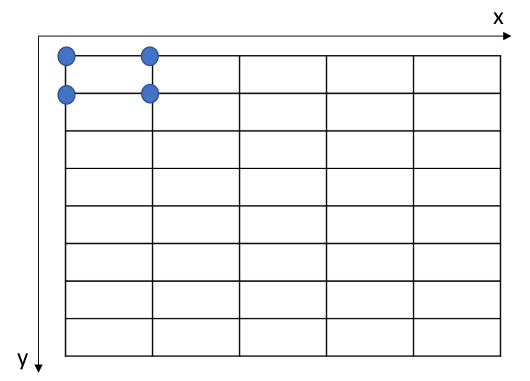
\includegraphics[width=2.5in]{figures/twoagent1.png}
  \caption{Arrangement of agents at the beginning(when $a=2$)}\label{fig:twoagent1}
\end{figure}
Now let's consider the routes for the agents. For convenience, we assume that all the agents move at $T(x)\,(x\in\mathbb{Z}^*)$ because some time should be reserved for the coordination after the BV is triggered. More detail about the moving cycle would be discussed after we decide the number of agents and the routes for them. 
Let $v=(x, y)$ be the node under exploration, with $1\leq x_i \leq d_1$, $1\leq i \leq d_2$. Additionally, we define ``Vertical Moving Mark'' (VMM) for every agent: VMM can only change between $0$ and $1$; every time when the agent moves SOUTH, that value changes. For example, if one agent continues to move SOUTH at $T(x)\,(x\in\mathbb{Z}^*)$ and its $Vertical_D$ is originally $0$, then its $Vertical_D$ changes into $1$ at $T(1)$, $0$ at $T(2)$ and so on.
Every agent hold two VMMs in its memory and let's say $VMM_1$ and $VMM_2$. The original value of $VMM_1$ of the agents is $0$; the original value of $VMM_2$ of agents residing at node $(1, y)$ and node $(2, y)$ ($1\leq y\leq a$) is $0$ and $1$ respectively. 

we now define the action of the $2a\,(a\in\mathbb{Z}^*)$ agents:\\ 
\begin{itemize}
\item Let $b=a-1$. When all agents' $VMM_1$ are ``0", then those agents with $VMM_2$ equal to ``0" move EAST when $x\neq d_1-1$ and move SOUTH for $b$ steps when $x=d_1-1$; those agents with $VMM_2$ equal to ``1" move EAST when $x\neq d_1$ and move SOUTH for $b$ when $x=d_1$. When all agents' $VMM_1$ are ``0", then those agents with $VMM_2$ equal to ``0"  move WEST when $x\neq2$ and move SOUTH for $b$ steps when $x=2$; those agents with $VMM_2$ equal to ``1" move WEST when $x\neq 1$ and move SOUTH for $b$ steps when $x=1$.
\item A agent only move to a node which it has not explored. (Note that when residing at a node, a agent is able to know whether it has explored the neighbours of that node or not.)
\end{itemize}
Informally, the routes of agents are snakelike routes. When $a=2$, the routes of agents are shown as Fig\ref{fig:twoagent2}.
%\iffalse
\begin{figure} [H]
  \centering 
  \subfigure[Routes of agents in the first line when $a=2$]{ 
    \label{fig:agentroute:a} %% label for first subfigure 
    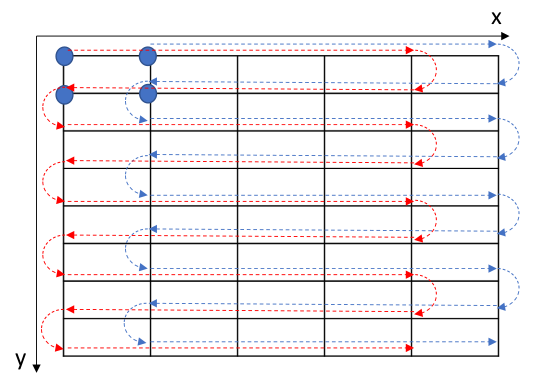
\includegraphics[width=3.5in]{figures/twoagentroute1.png}} 
 \hspace{1in} 
  \subfigure[Routes of agents in the second line when $a=2$]{ 
    \label{fig:agentroute:b} %% label for second subfigure 
    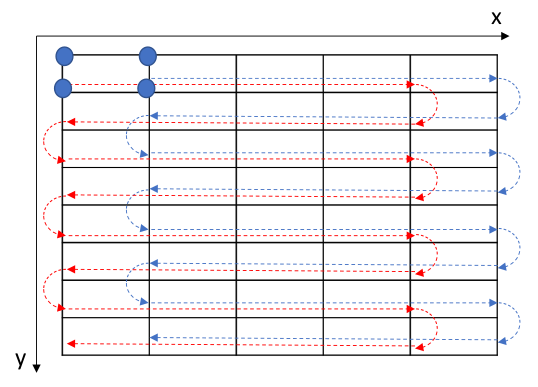
\includegraphics[width=3.5in]{figures/twoagentroute2.png}}
  \caption{Routes of agents when $a=2$} 
  \label{fig:twoagent2} %% label for entire figure 
\end{figure}
%\fi


when $a=3$, the routes of agents are shown as Fig\ref{fig:threeagent1}. 
\begin{figure} [H]
  \centering 
  \subfigure[Routes of agents in the first line when $a=3$]{ 
    \label{fig:agentroute:a} %% label for first subfigure 
    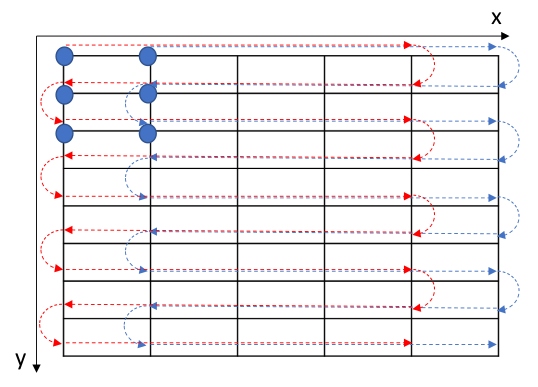
\includegraphics[width=3.5in]{figures/threeagentroute1.png}} 
  \hspace{1in} 
  \subfigure[Routes of agents in the second line when $a=3$]{ 
    \label{fig:agentroute:b} %% label for second subfigure 
    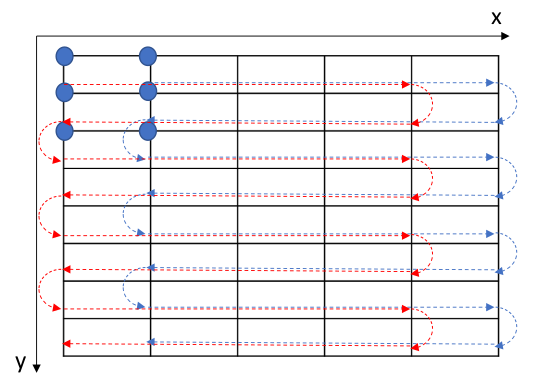
\includegraphics[width=3.5in]{figures/threeagentroute2.png}}
    \hspace{1in} 
    \subfigure[Routes of agents in the second line when $a=3$]{ 
    \label{fig:agentroute:c} %% label for second subfigure 
    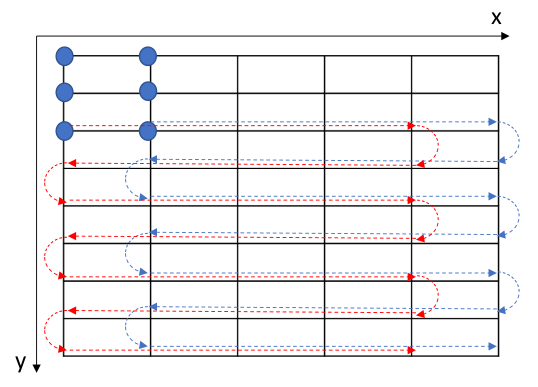
\includegraphics[width=3.5in]{figures/threeagentroute3.png}}
  \caption{Routes of agents when $a=3$} 
  \label{fig:threeagent1} %% label for entire figure 
\end{figure}





Initially, 2$d_1$ agents are placed at the first two columns at $T_0$. More specifically, the coordinate of them are (1, $x_i$) and (2,$x_i$) where $1\leq x_i\leq d_1$. The agents residing in the first column are in the shadowing group while the agents residing in the second column are in the exploring group. If the BV resides in a node in the first column, then all of its clones are destroyed. If the BV resides in a node in the second column, then the elimination phase begins. It is obvious that if the BV do not reside in any node in the first column, then a agent in the exploring group should be destroyed when the BV is exposed.  Let's assume that the we starts at $T_0$. Agents residing in nodes in the second column moves EAST at the beginning of T(2n), $n=0,1, \ldots ,d_2-1$. More precisely, node (x, y) move to (x+1, y) at the beginning of T(2n), $n=0,1, \dots , d_2-1$. Agents residing in the first column simply follow the node in the second column (see  Fig.\ref{fig:TShE}). When one of the node in the former column is destroyed by a BV, the second phase starts.
\begin{figure}[H]
  \centering  
  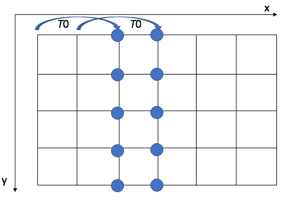
\includegraphics[width=2.5in]{figures/TShE.png}
  \caption{Agents move at time $T_0$}\label{fig:TShE}
\end{figure}
\noindent{\bf Elimination Phase}\\
The elimination begins when one of the node in the former column is destroyed by a BV( let's say, at T(2$x_i$)). No matter where is the BV, there are always three agents residing on its north(if the BV is not in the first line), west and south (if the BV is not in the last line), so only one BV clone survives. In another word, only one node becomes BV node after the BV being triggered.  Observe that in the parallel strategy, not all agents participate in the elimination phase automatically when the BV is explored because only those receive the clones of the original BV and those be notified by other agents can participate in the elimination phase. Since we want to make use of the agents we employ at the beginning in the elimination phase which means the situation that the number of agents is not enough for completing the elimination phase but there are still some agents keeping exploring the graph is not allowed to happen. So in some situation, agents who receive the BV clone should notify other agents to participate in the elimination.  Let the node where the surviving clone resided be $(x, y)$ and its situation can be divided into four cases. Different routes of agents in the elimination phase are based on the location of the new formed BV.
\begin{itemize}
\item Case 1: When $2<x<d_1$, $1<y<d_2-1$ (a interior node becomes a new formed BV), then agents (let's say agents $a,b,c$) residing in node $(x-1, y+1)$, $(x-1, y-1)$ and $(x-2, y)$ receive a BV clone at T(2$x_i$+1), so that they know the location of the original BV and also the new formed BV. Note that in the exploring phase, the agents move EAST at T(2n), $n=0,1, \ldots ,d_2-2$. Actually, one unit of time is reserved for some agents to receive the BV clone. After they receive the BV clone, these agents move EAST for one step (for example, to node $(x, y+1)$, $(x, y-1)$ and $(x-1, y)$ and stop. Note that other agents including agents residing in node $(x-2, y+1)$ and $(x-2, y-1)$ (let's say agent d and e) at T(2$x_i$) do not know the existence of the BV so they keep moving EAST. These two agents arrive at nodes $(x, y+1)$, $(x, y-1)$ at T(2($x_i+2$)) and at this time they meet agent $a$ and $b$ respectively. Agent $a$ and $b$ inform them of the location of the new form BV and the routes of agents $d$ and $e$ are as follow:\\
route of $d$: $(x, y+1)(at\ T(2(x_i+2)){\rightarrow}(x+1,y+1)(at\ T(2(x_i+2)+1){\rightarrow}(x+1,y)(at\ T(2(x_i+3))$.\\
route of $e$: $(x, y-1)(at\ T(2(x_i+2)){\rightarrow}(x, y)(at\ T(2(x_i+3)+1))$.
The routes of agents are showed in Fig.\ref{fig:subfigmesh1} where a blue node indicate that there are one agent residing here; a red node indicate that there are two agents residing here; a yellow node indicate that there are three agents residing here.

%\iffalse
\begin{figure} [H]
  \centering 
  \subfigure[$T(2x_i+1)$]{ 
    \label{fig:subfigmesh1:a} %% label for first subfigure 
    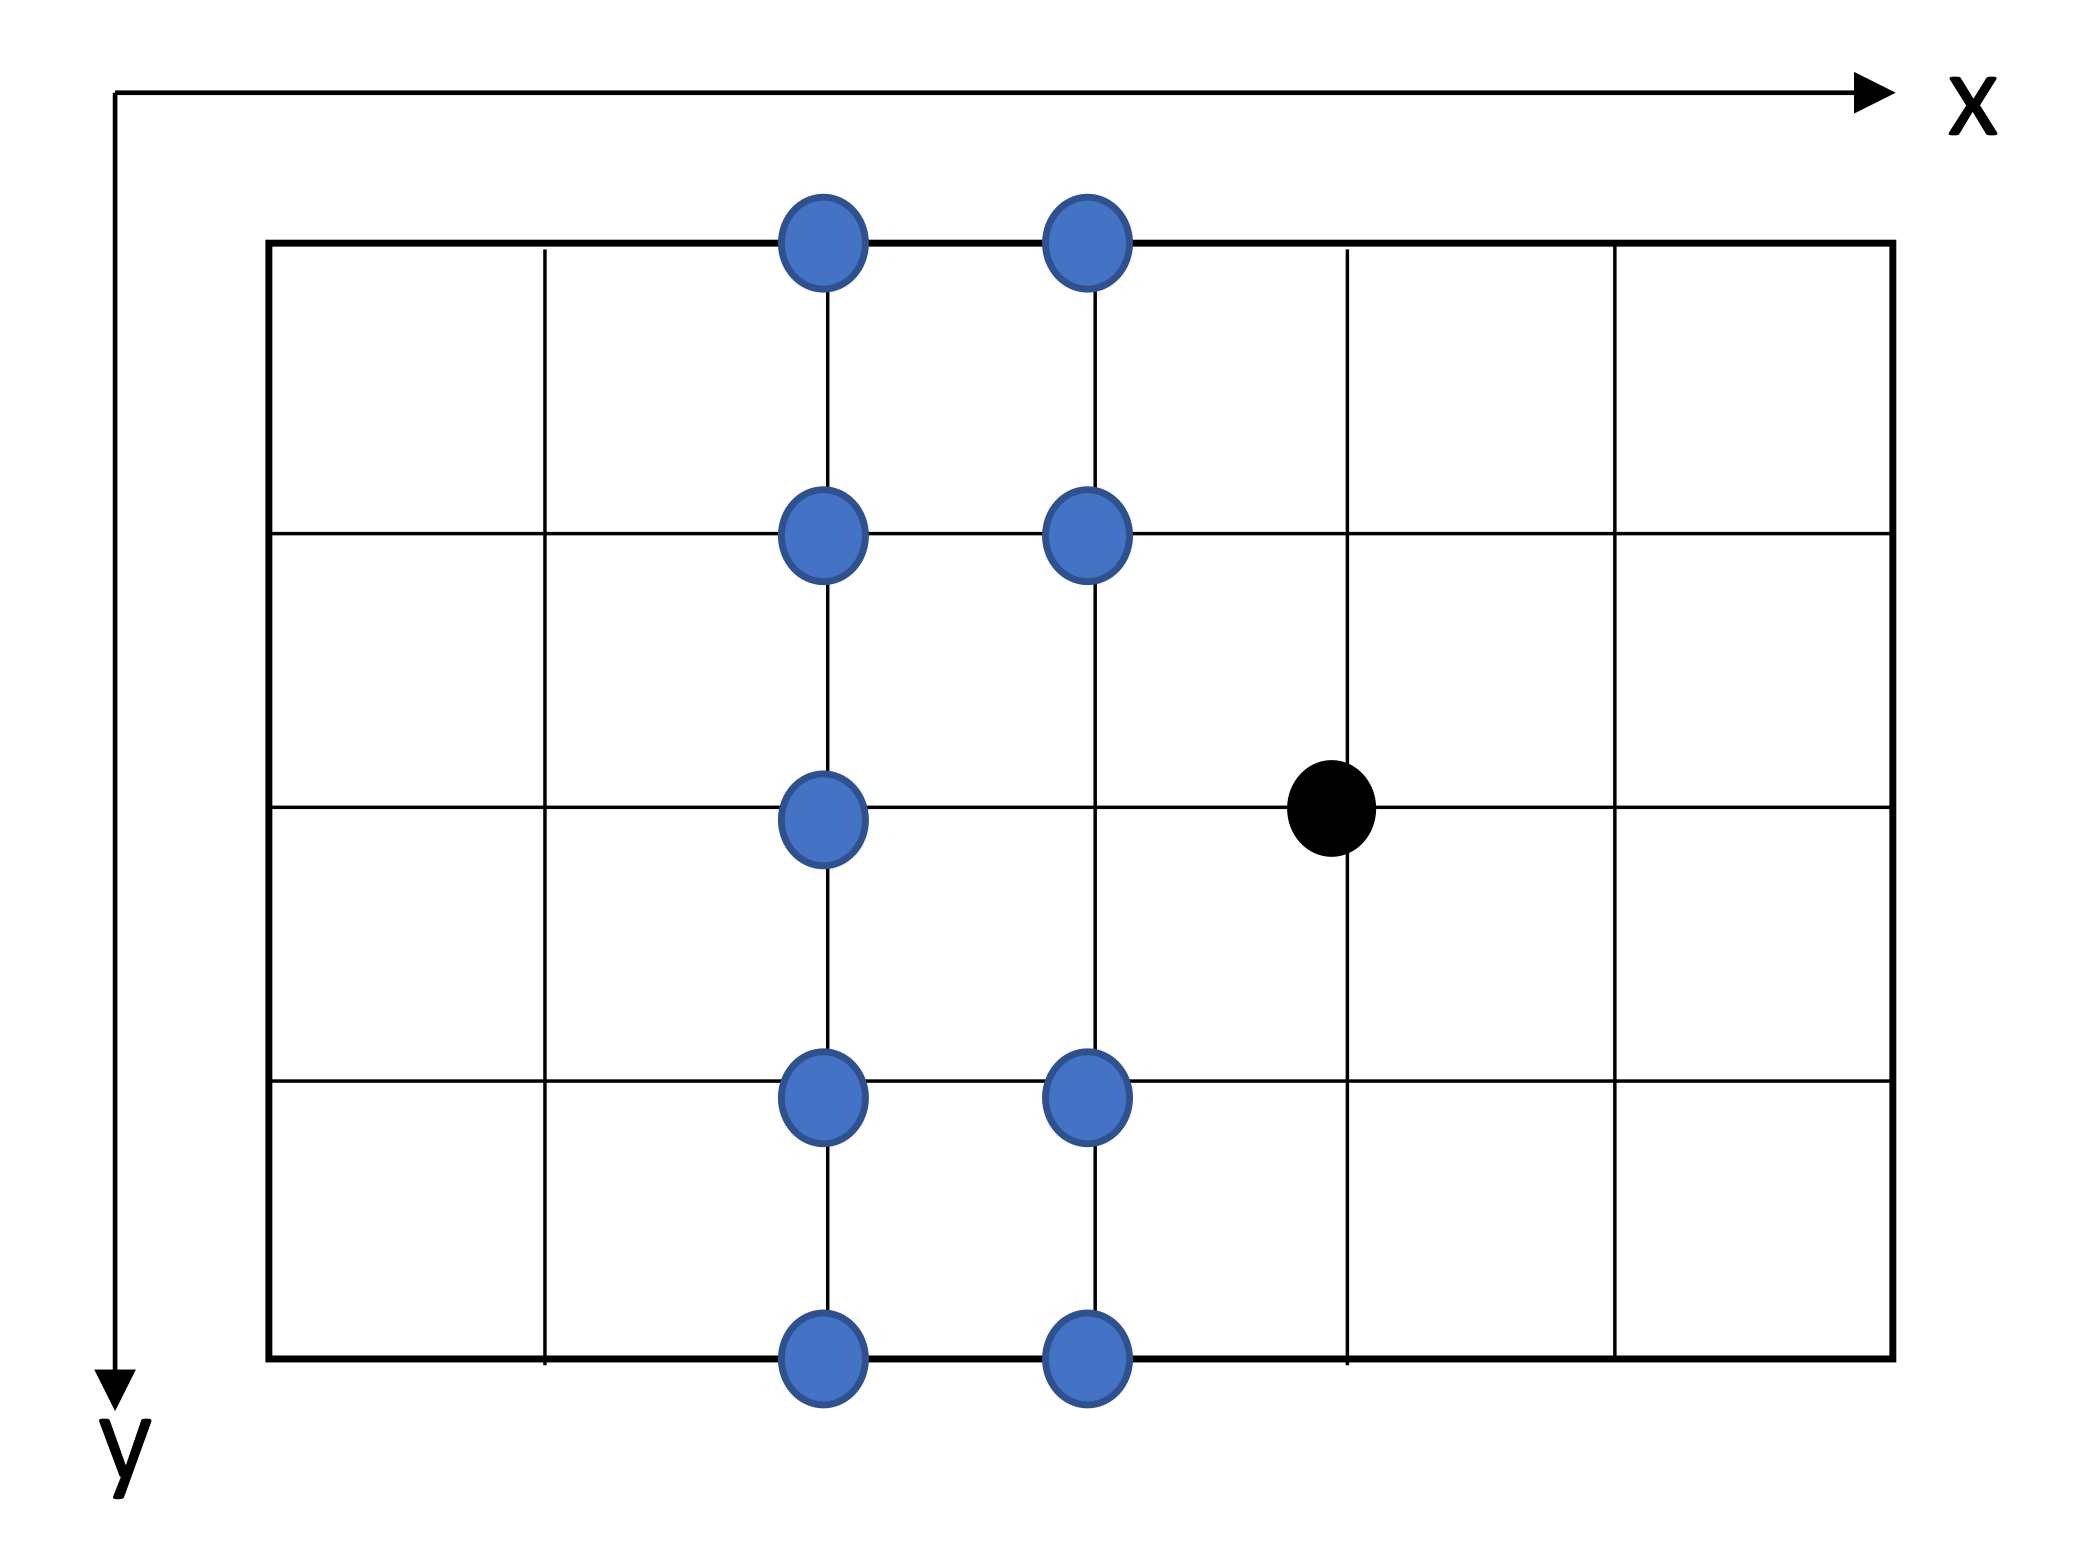
\includegraphics[width=2.5in]{figures/meshinterior.png}} 
%  \hspace{1in} 
  \subfigure[$T(2(x_i+1))$]{ 
    \label{fig:subfigmesh1:b} %% label for second subfigure 
    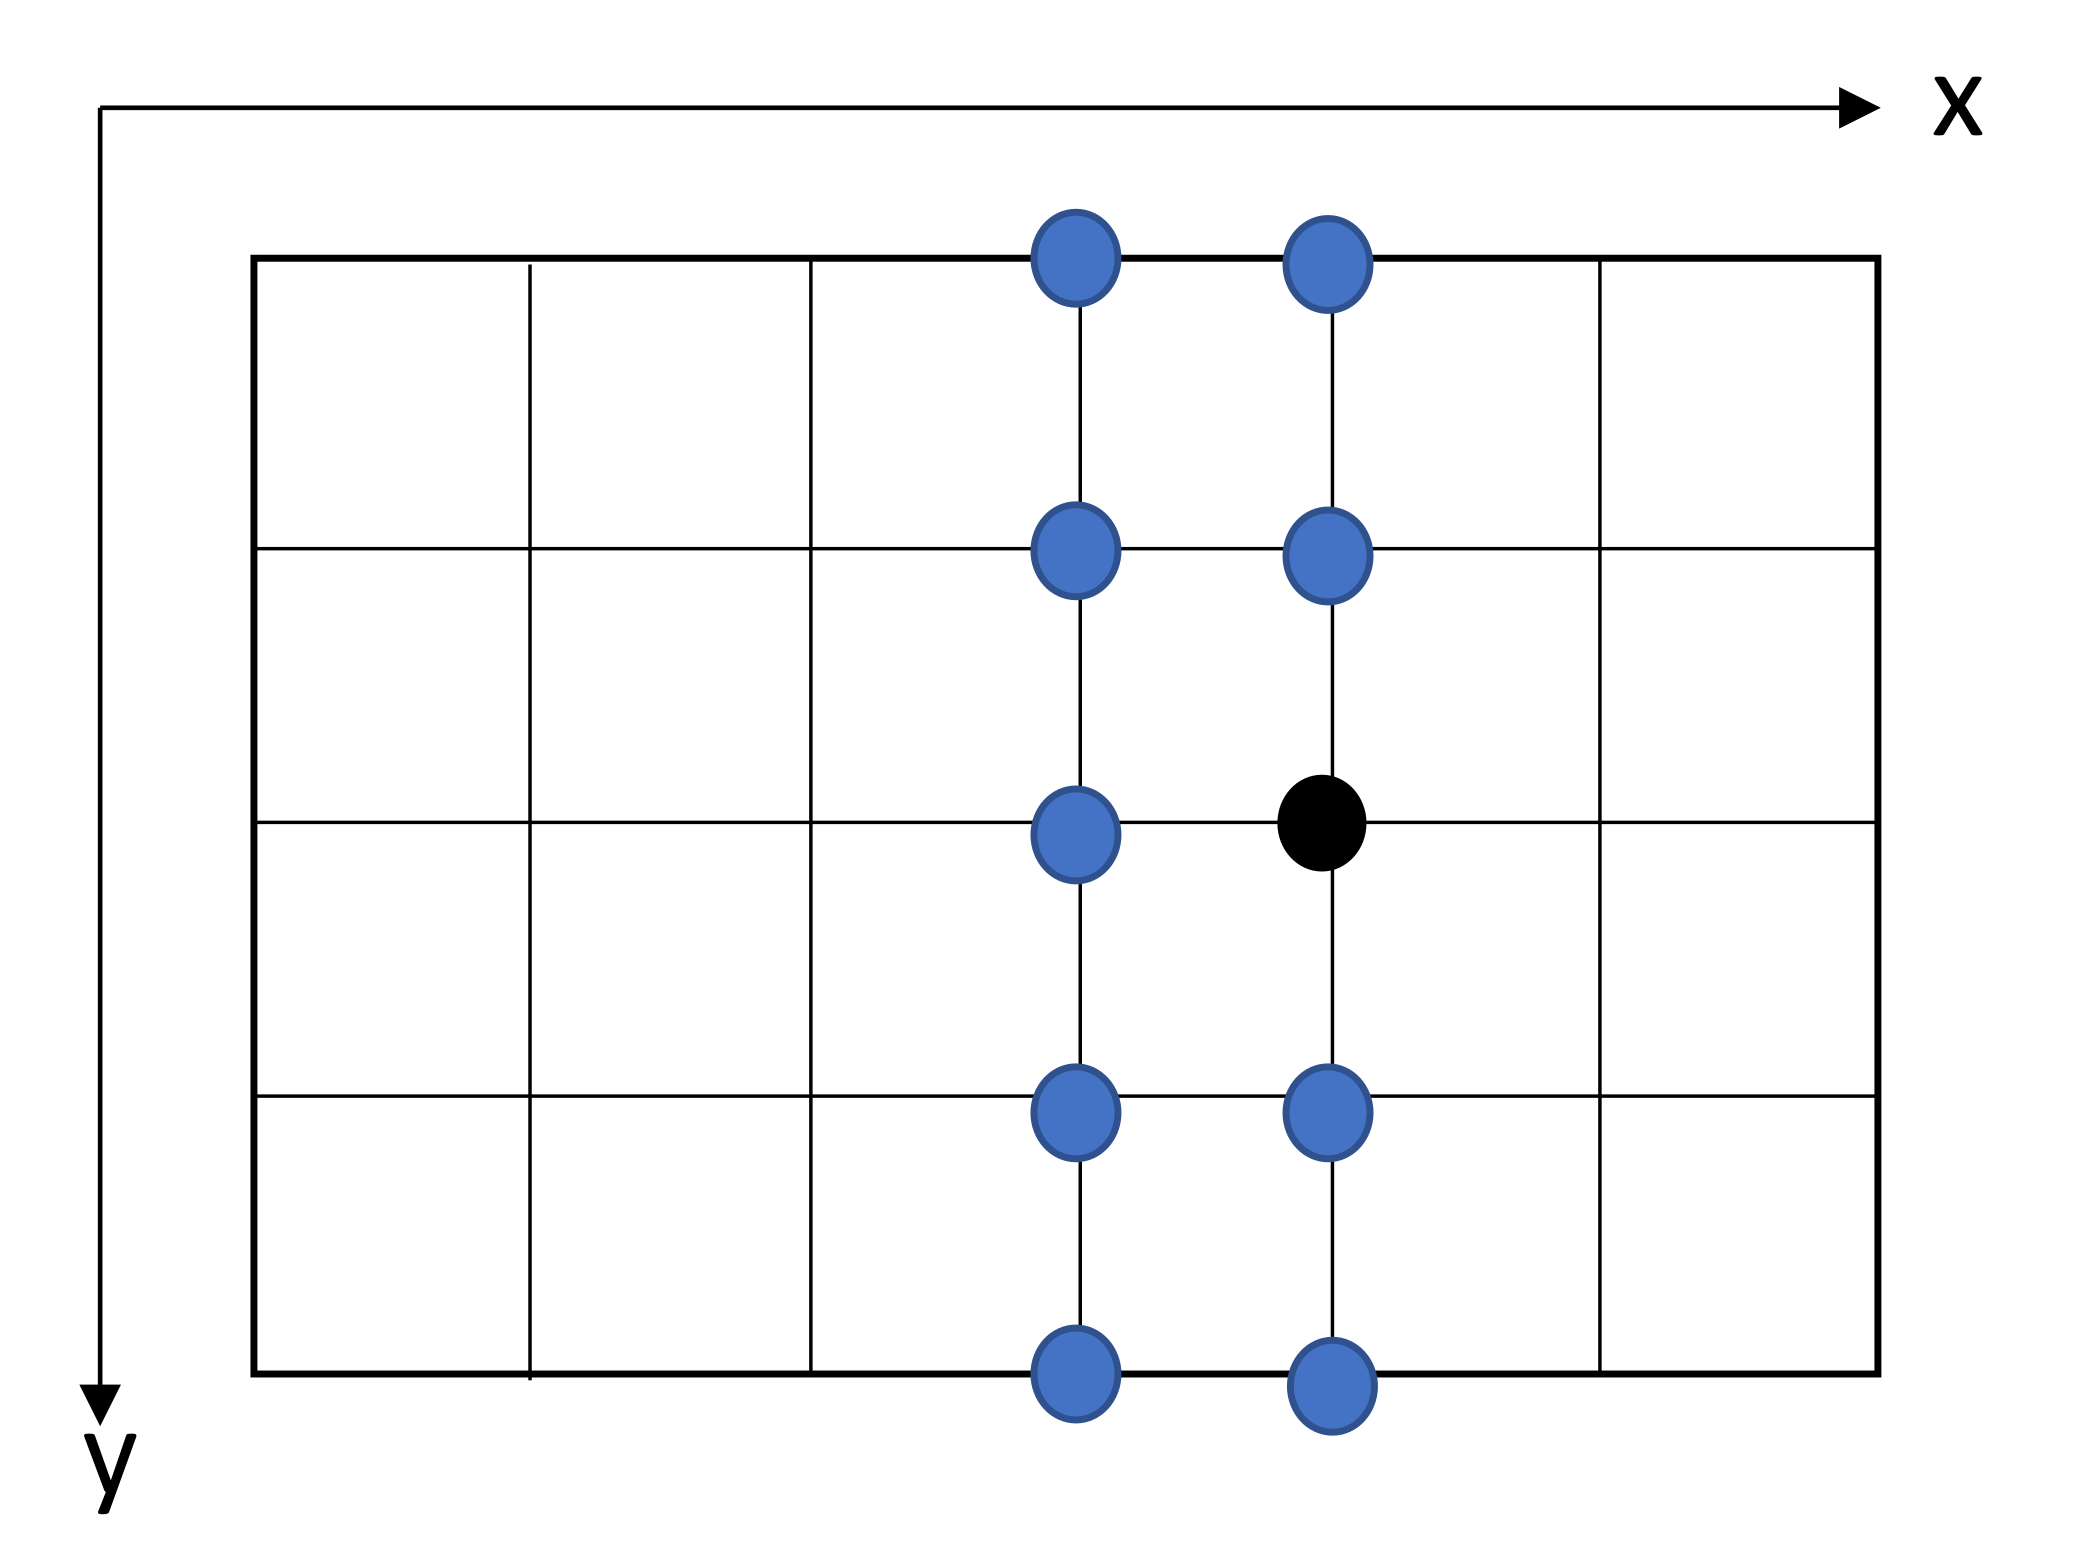
\includegraphics[width=2.5in]{figures/meshinterior1.png}}
    \hspace{1in} 
  \subfigure[$T(2(x_i+2))$]{ 
    \label{fig:subfigmesh1:c} %% label for second subfigure 
    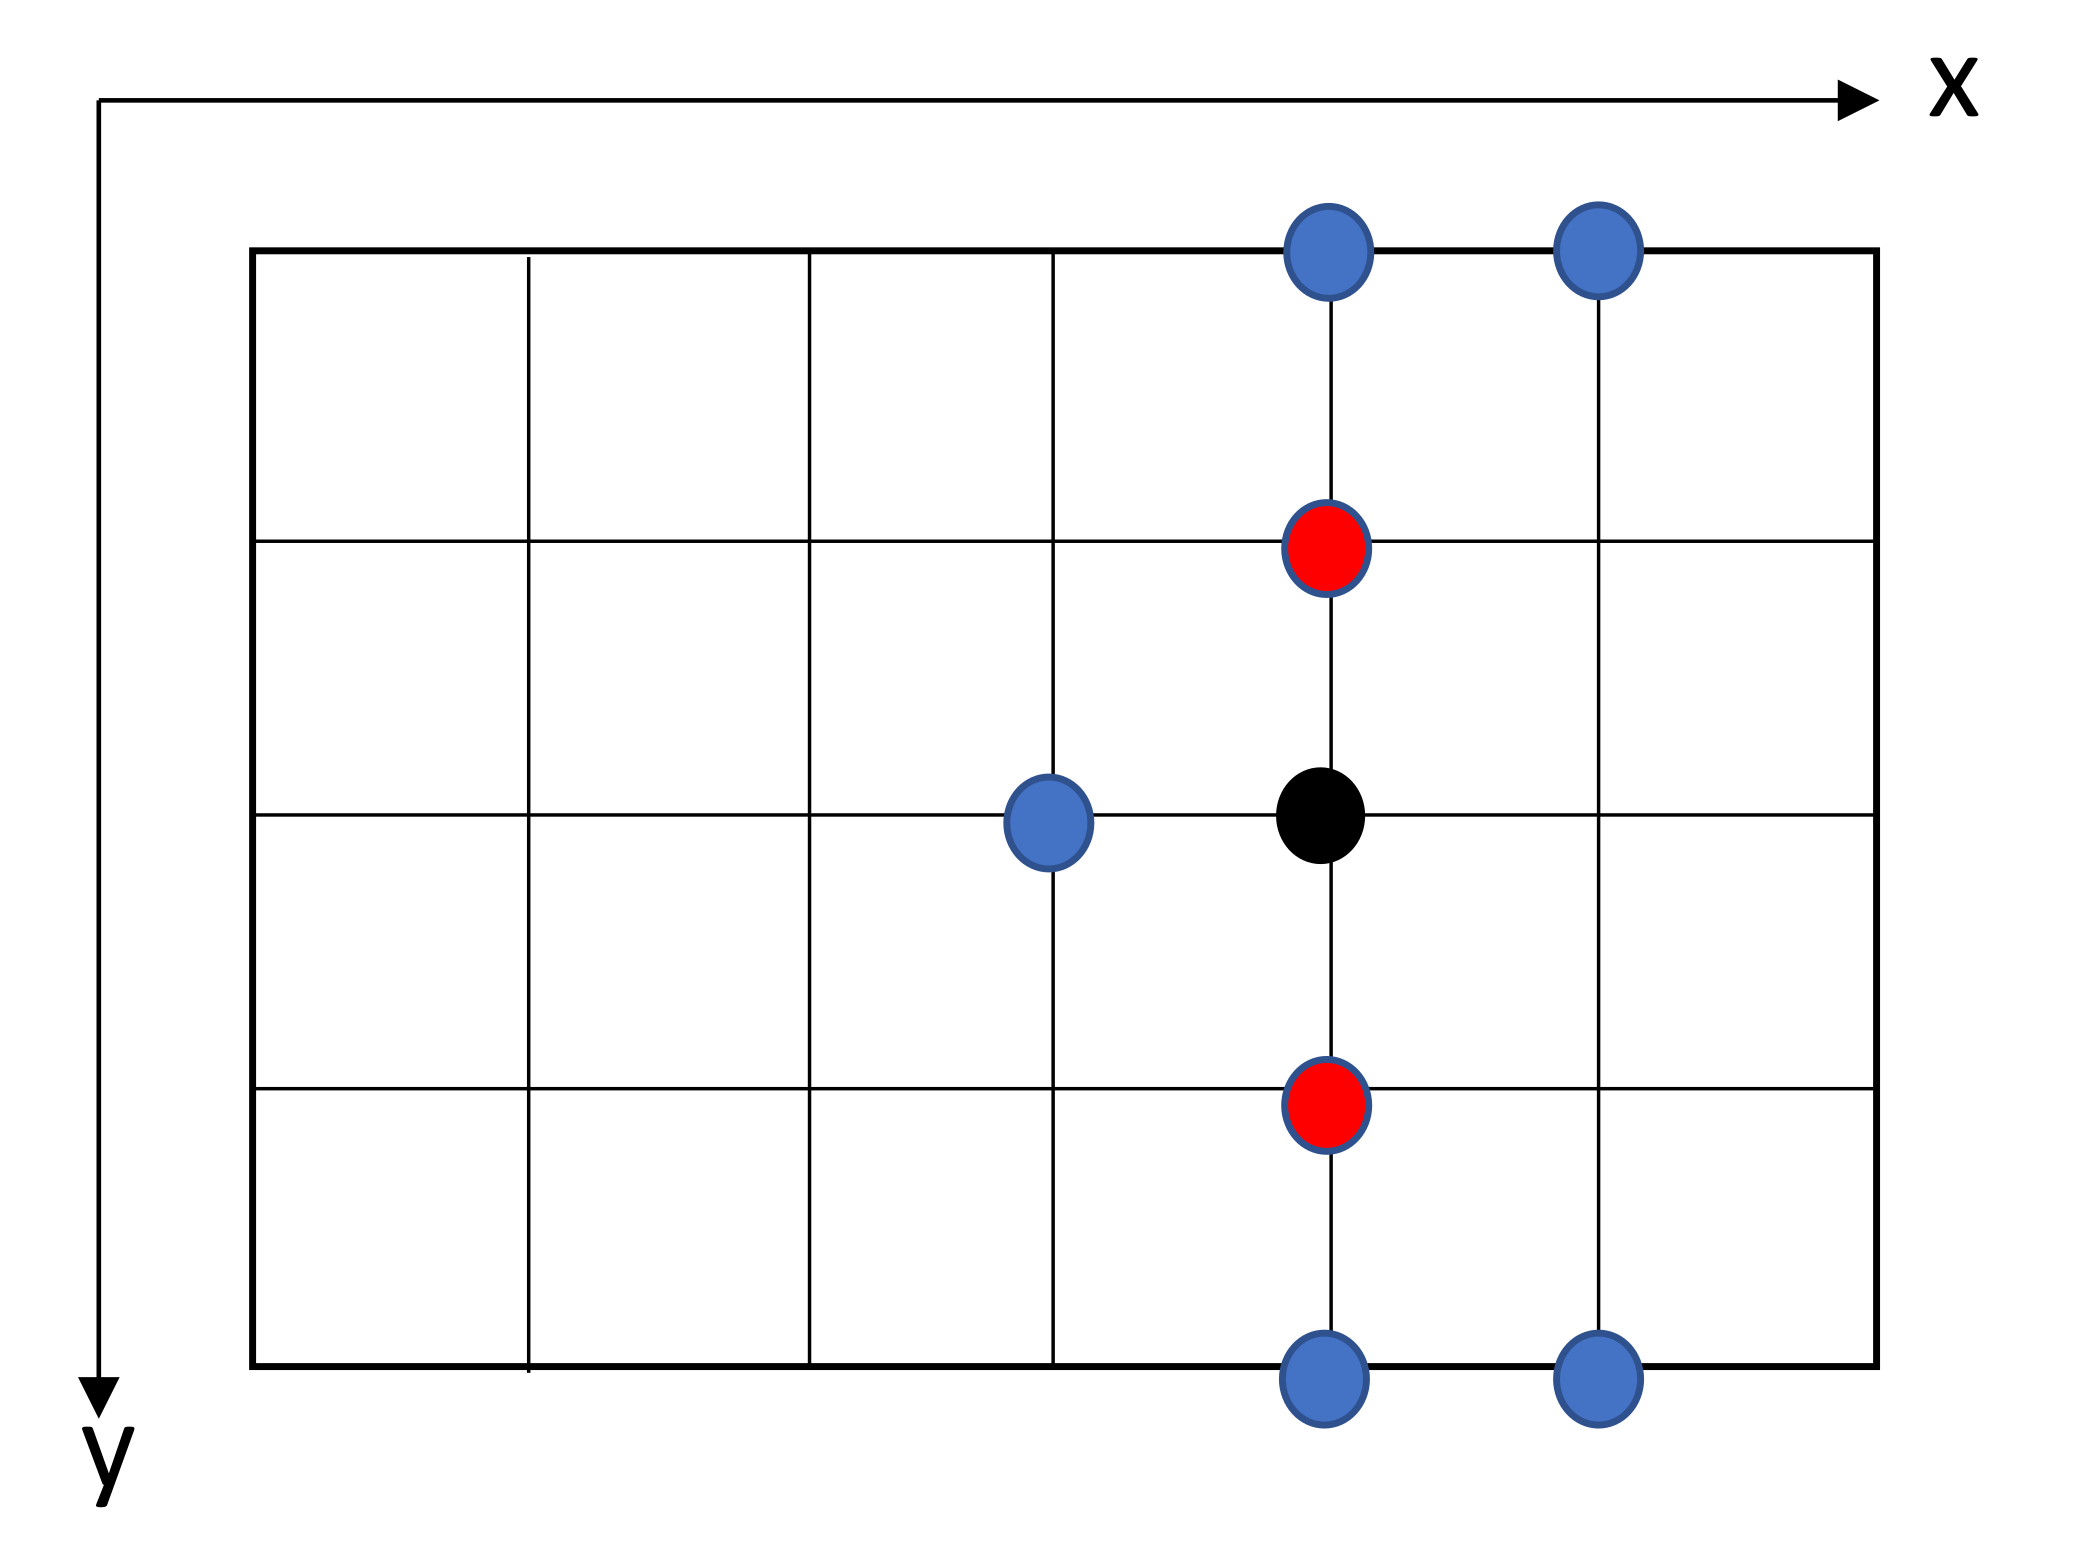
\includegraphics[width=2.5in]{figures/meshinterior2.png}}
%      \hspace{1in} 
  \subfigure[$T(2(x_i+3))$]{ 
    \label{fig:subfigmesh1:d} %% label for second subfigure 
    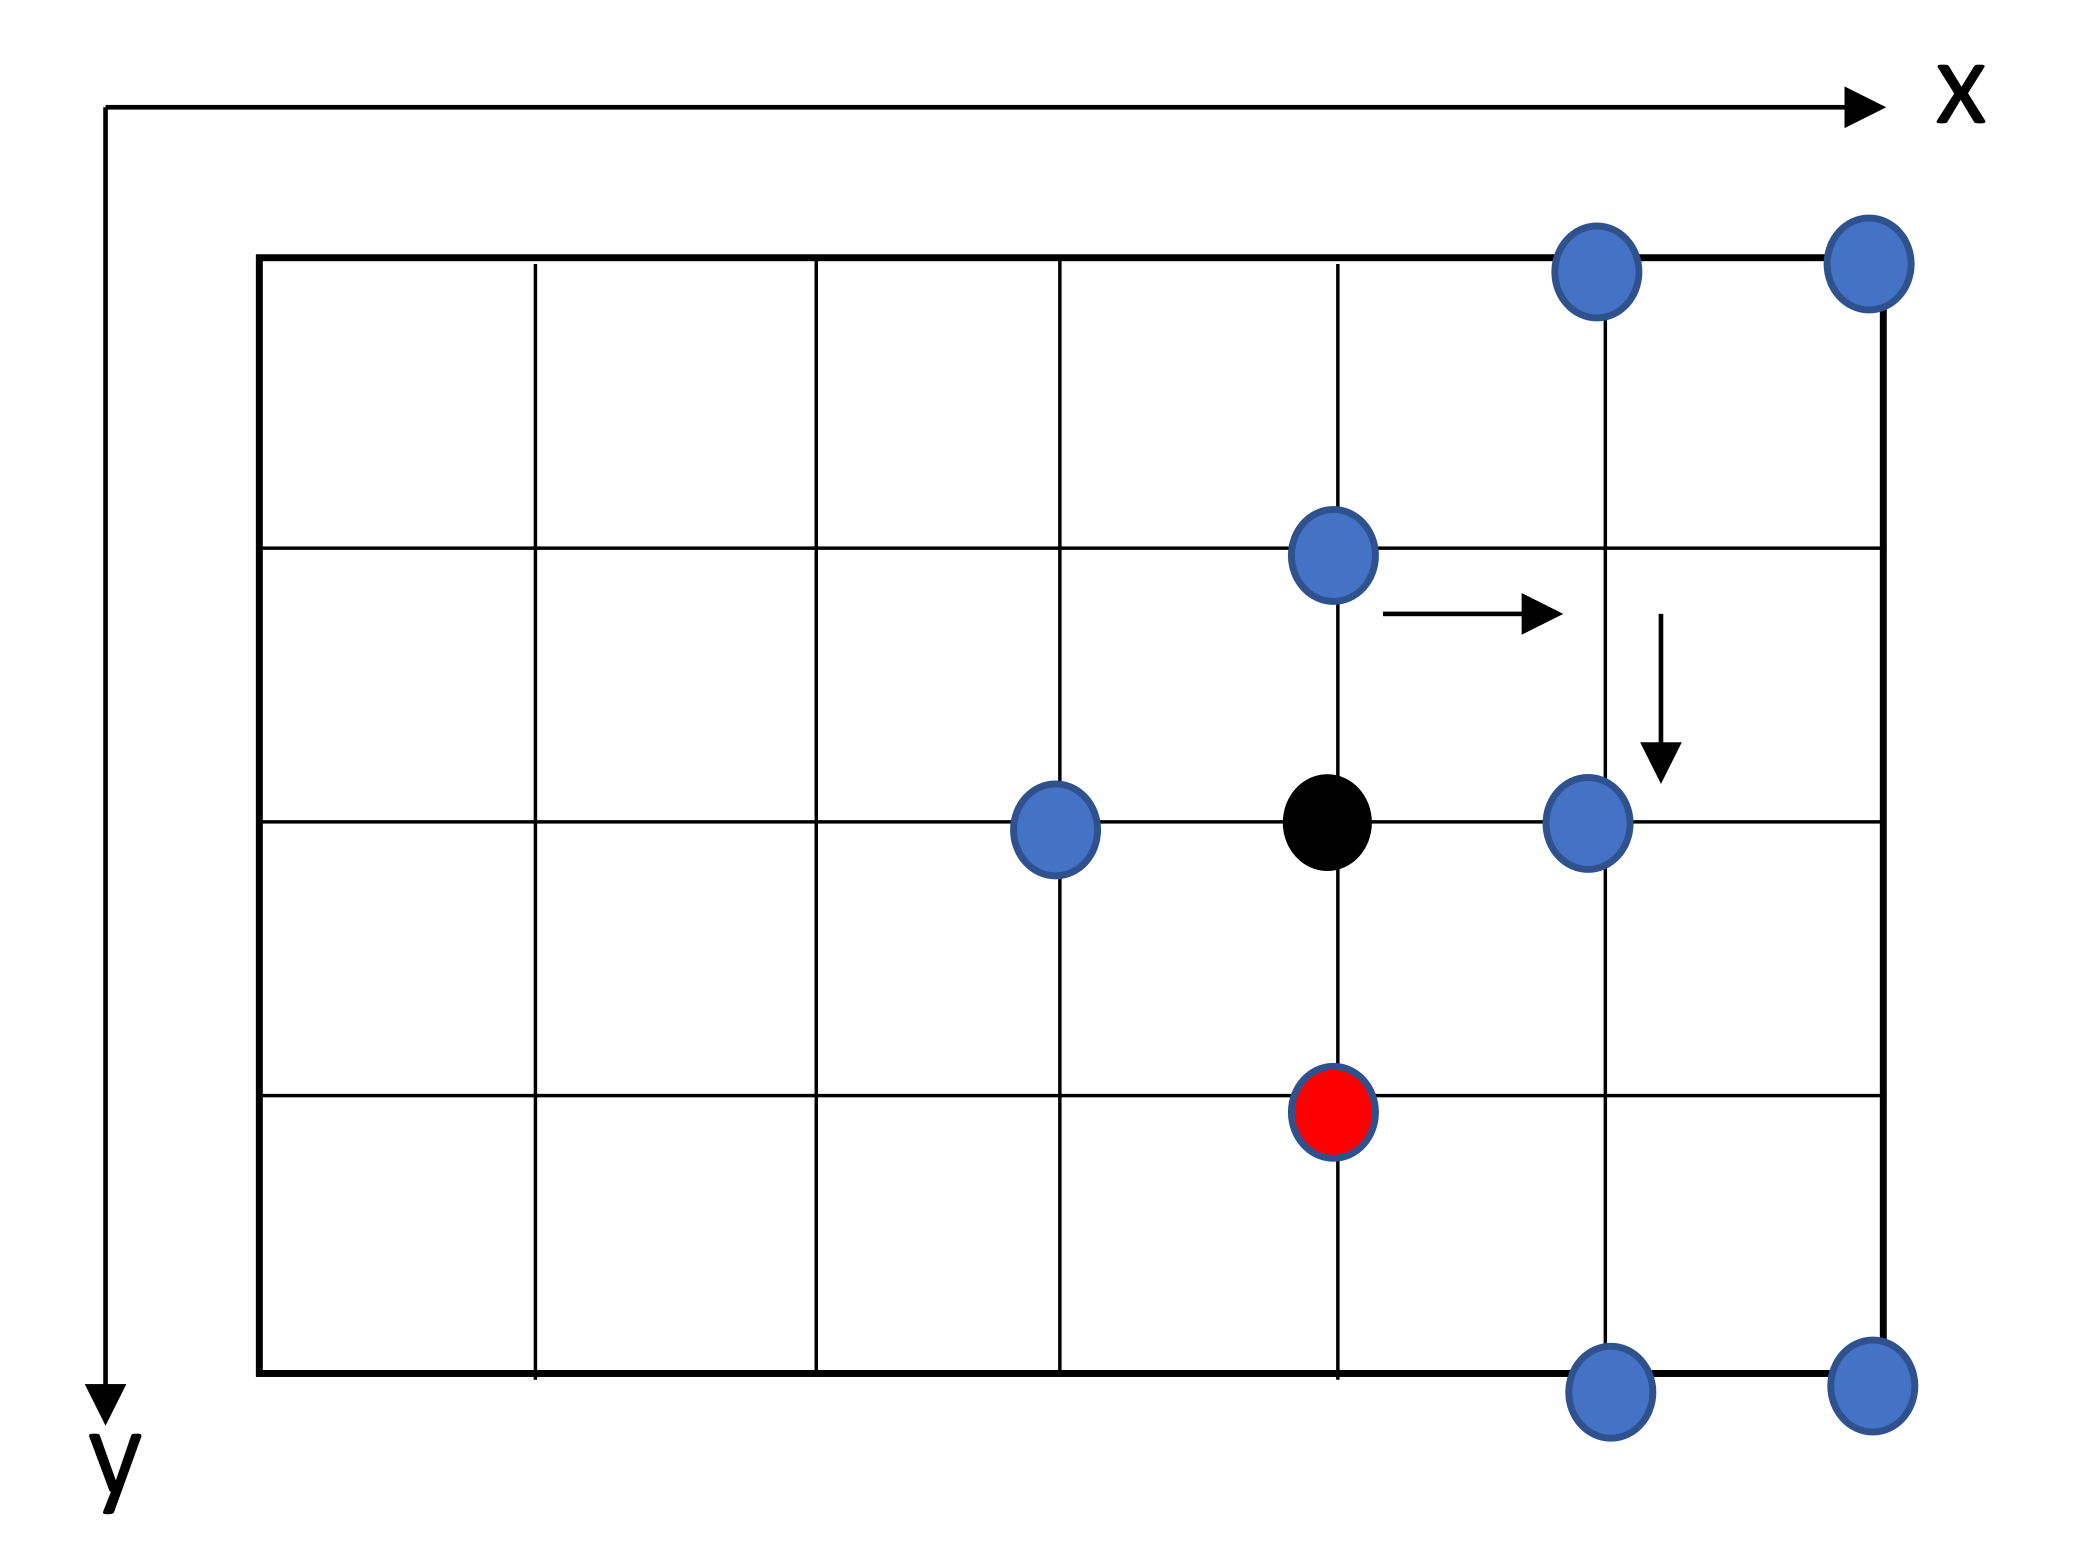
\includegraphics[width=2.5in]{figures/meshinterior3.png}}
      \hspace{1in} 
  \subfigure[$T(2(x_i+3)+1)$]{ 
    \label{fig:subfigmesh1:e} %% label for second subfigure 
    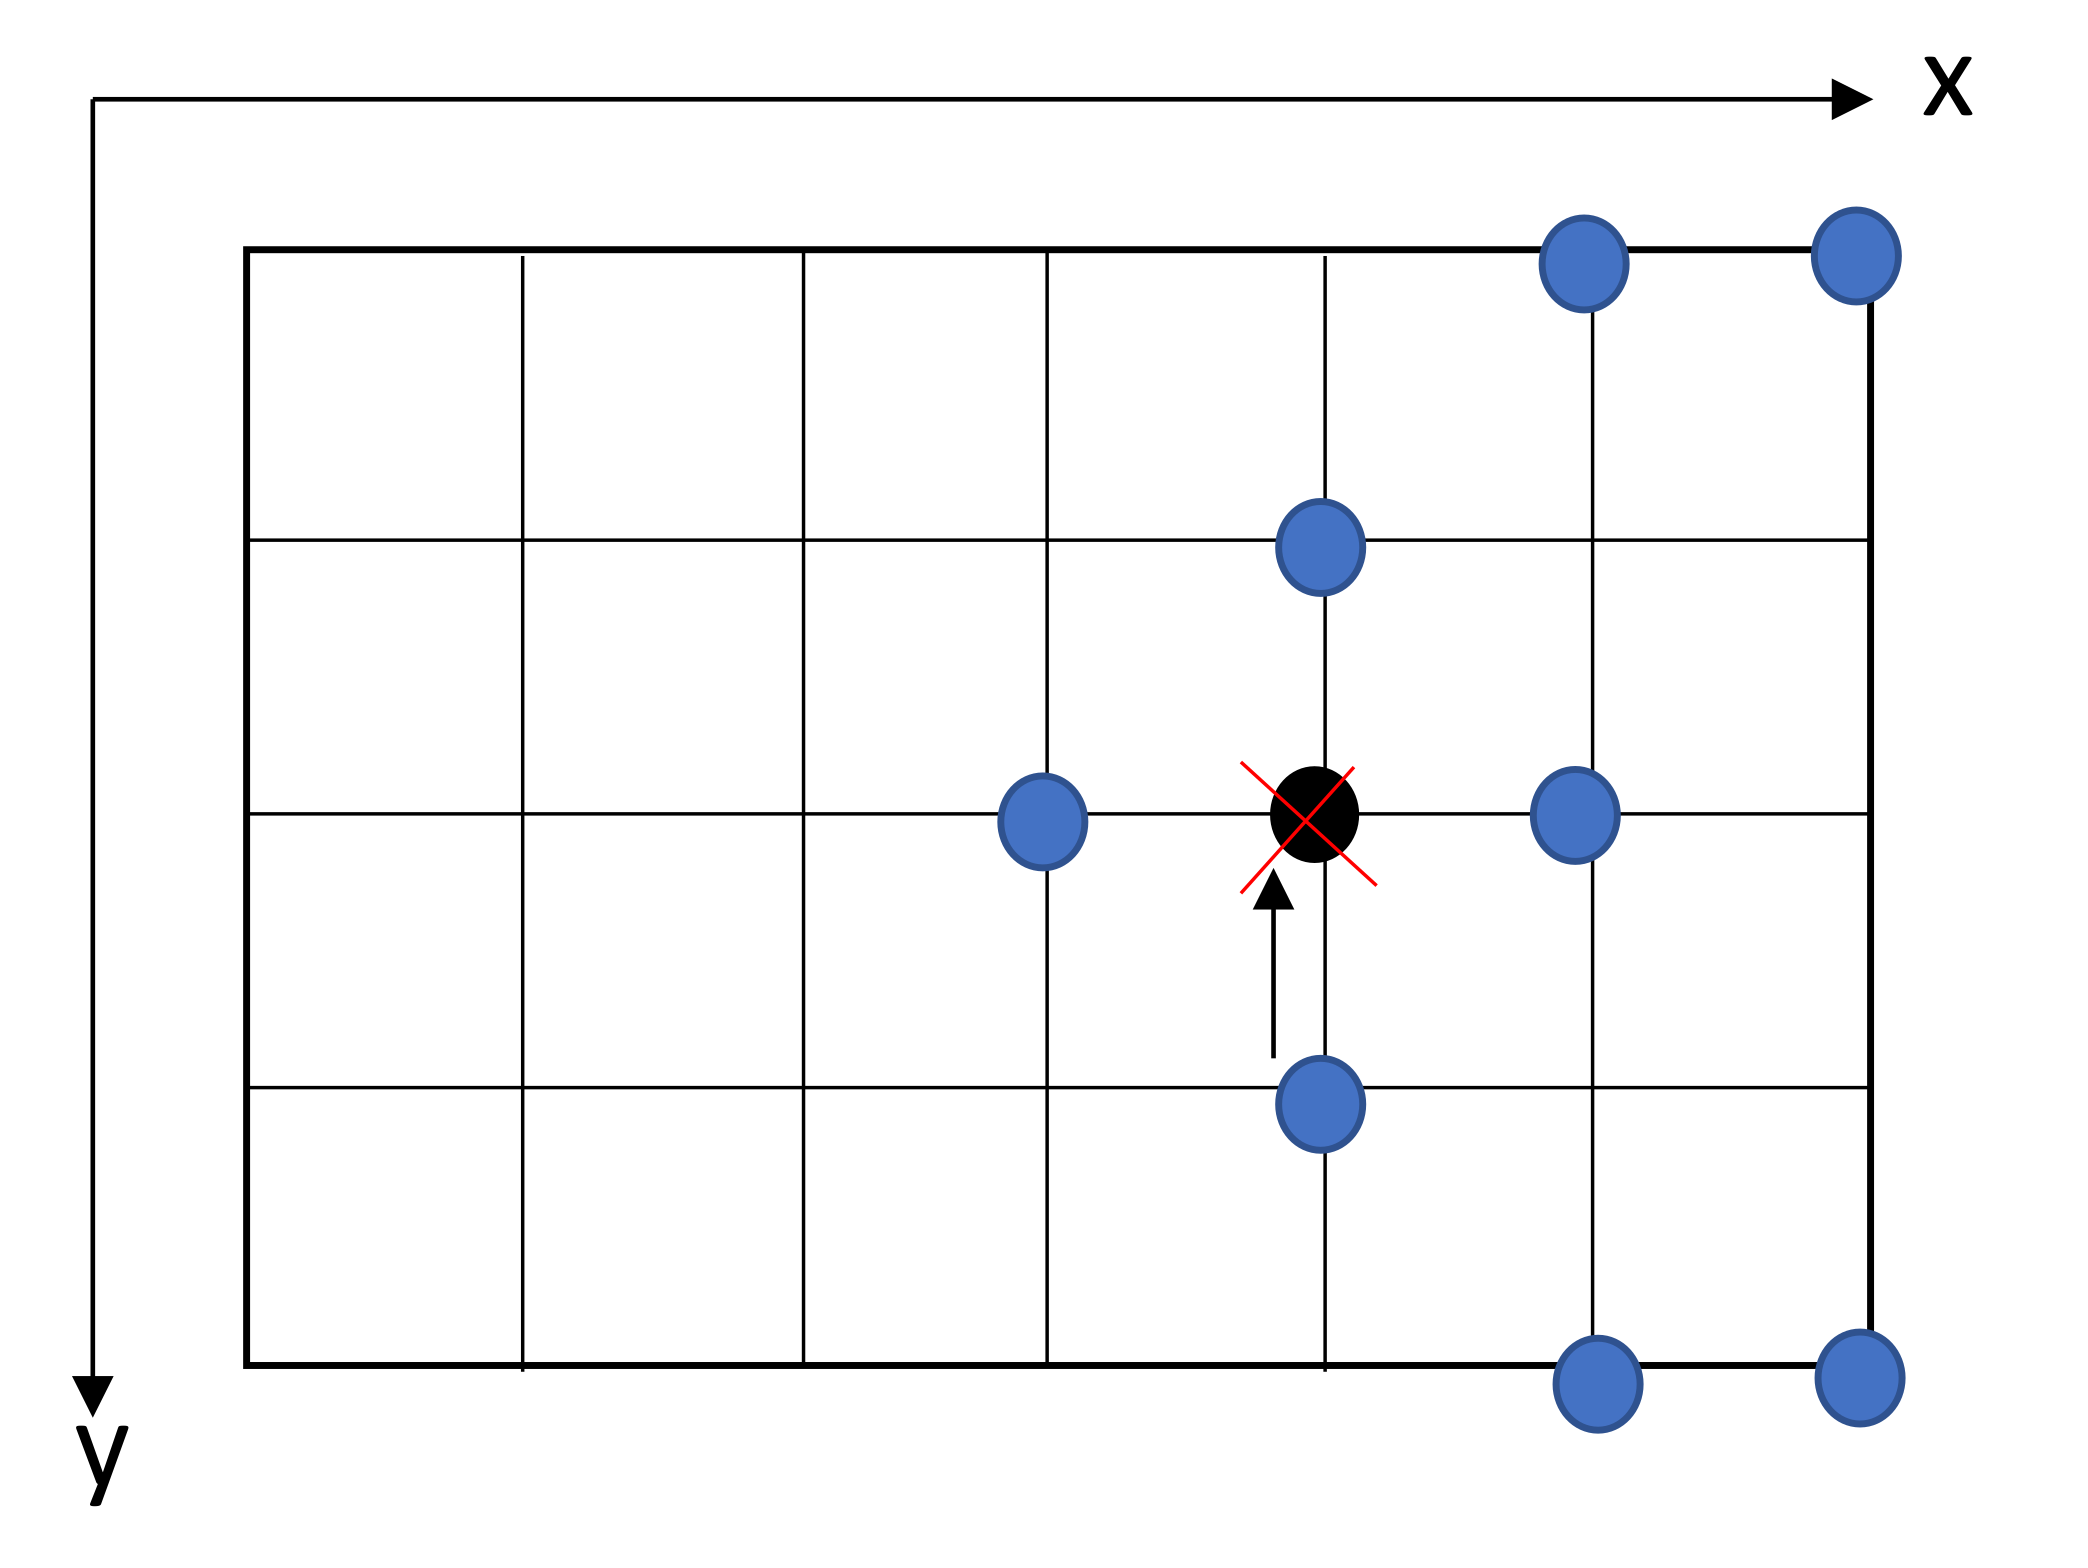
\includegraphics[width=2.5in]{figures/meshinterior4.png}}
  \caption{Arrangement of agents in elimination phase when the new formed BV resides in a interior node} 
  \label{fig:subfigmesh1} %% label for entire figure 
\end{figure}
%\fi


\item Case 2: When $x=d_1$, $2<y<d_2-1$ (a border node becomes a new formed BV), then agents (let's say agents $a,b,c$) residing in node $(x-1, y+1)$, $(x-1, y-1)$ and $(x-2, y)$ receive a BV clone at T(2$x_i$+1). As above, they move EAST for one step and stop. Agents residing in nodes $(x-2, y+1)$ and $(x-2, y-1)$ (let's say agents $a,b$) at T(2$x_i$) have no knowledge of the BV, so they keep moving and arrive at nodes $(x, y+1)$ and $(x, y-1)$ at T(2($x_i$+2)) when they are informed of the location of the new formed BV. One of agents $a$ and $b$ should move to the new formed BV to decontaminate it while the other one stop moving. In order to avoid conflict, we always employ the agent $a$ to move to the new formed BV.
\begin{figure} [H]
  \centering 
  \subfigure[$T(2x_i+1)$]{ 
    \label{fig:subfigmesh2:a} %% label for first subfigure 
    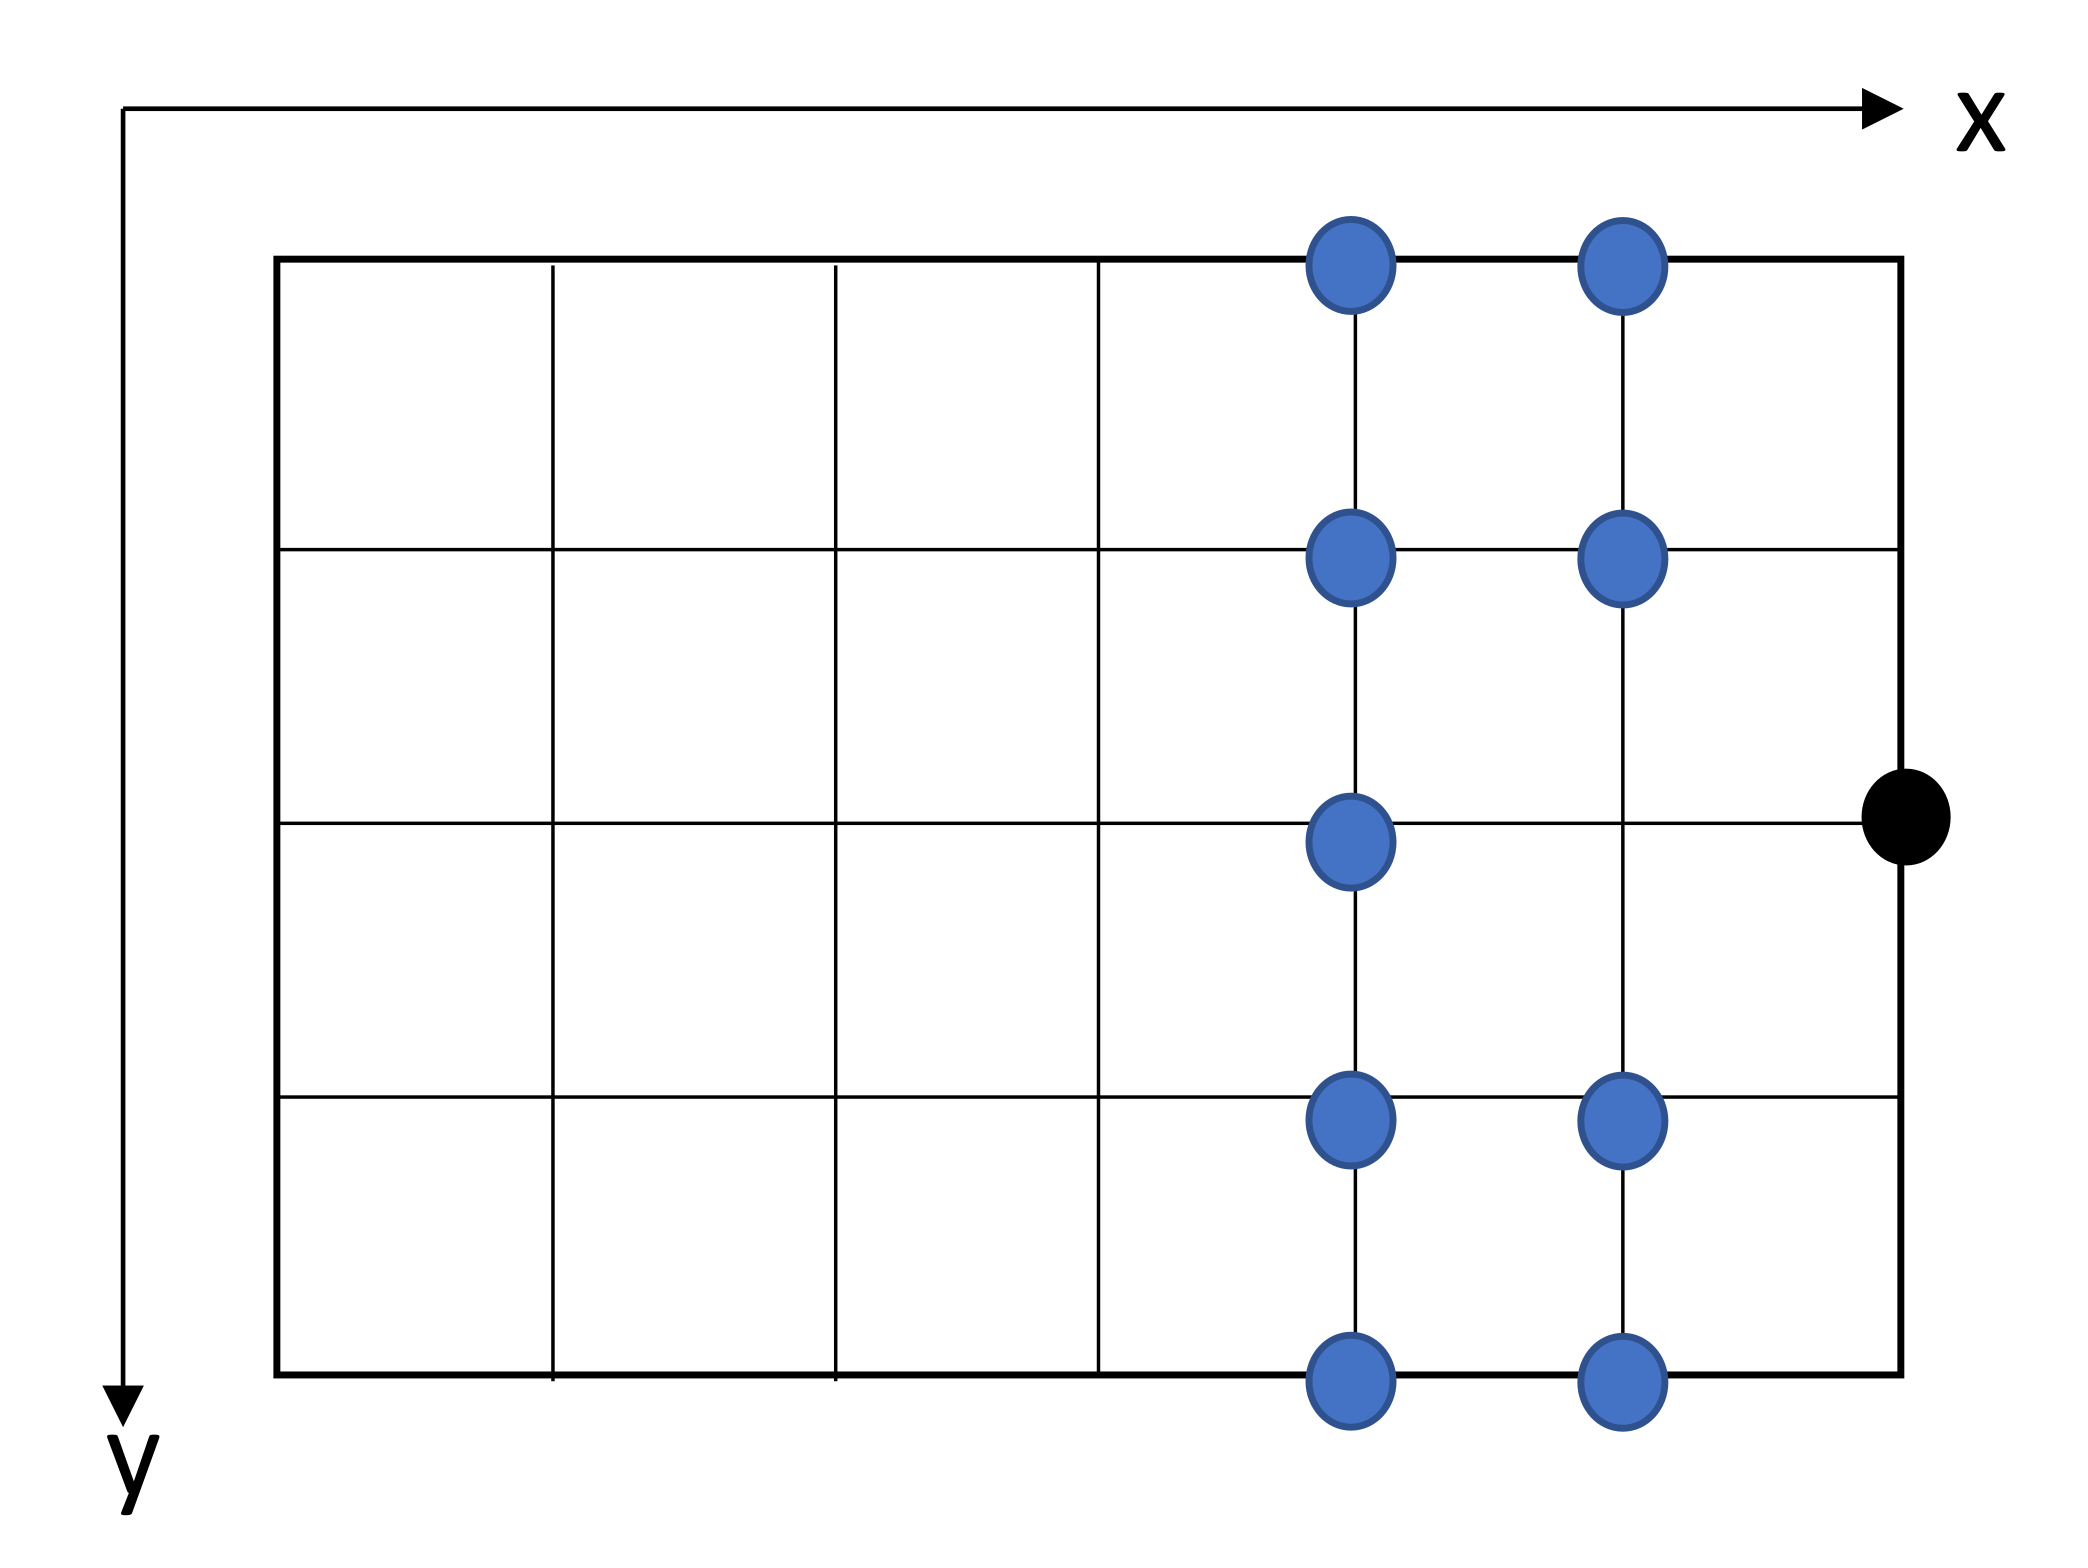
\includegraphics[width=2.5in]{figures/meshborderx1.png}} 
%  \hspace{1in} 
  \subfigure[$T(2(x_i+2))$]{ 
    \label{fig:subfigmesh2:b} %% label for second subfigure 
    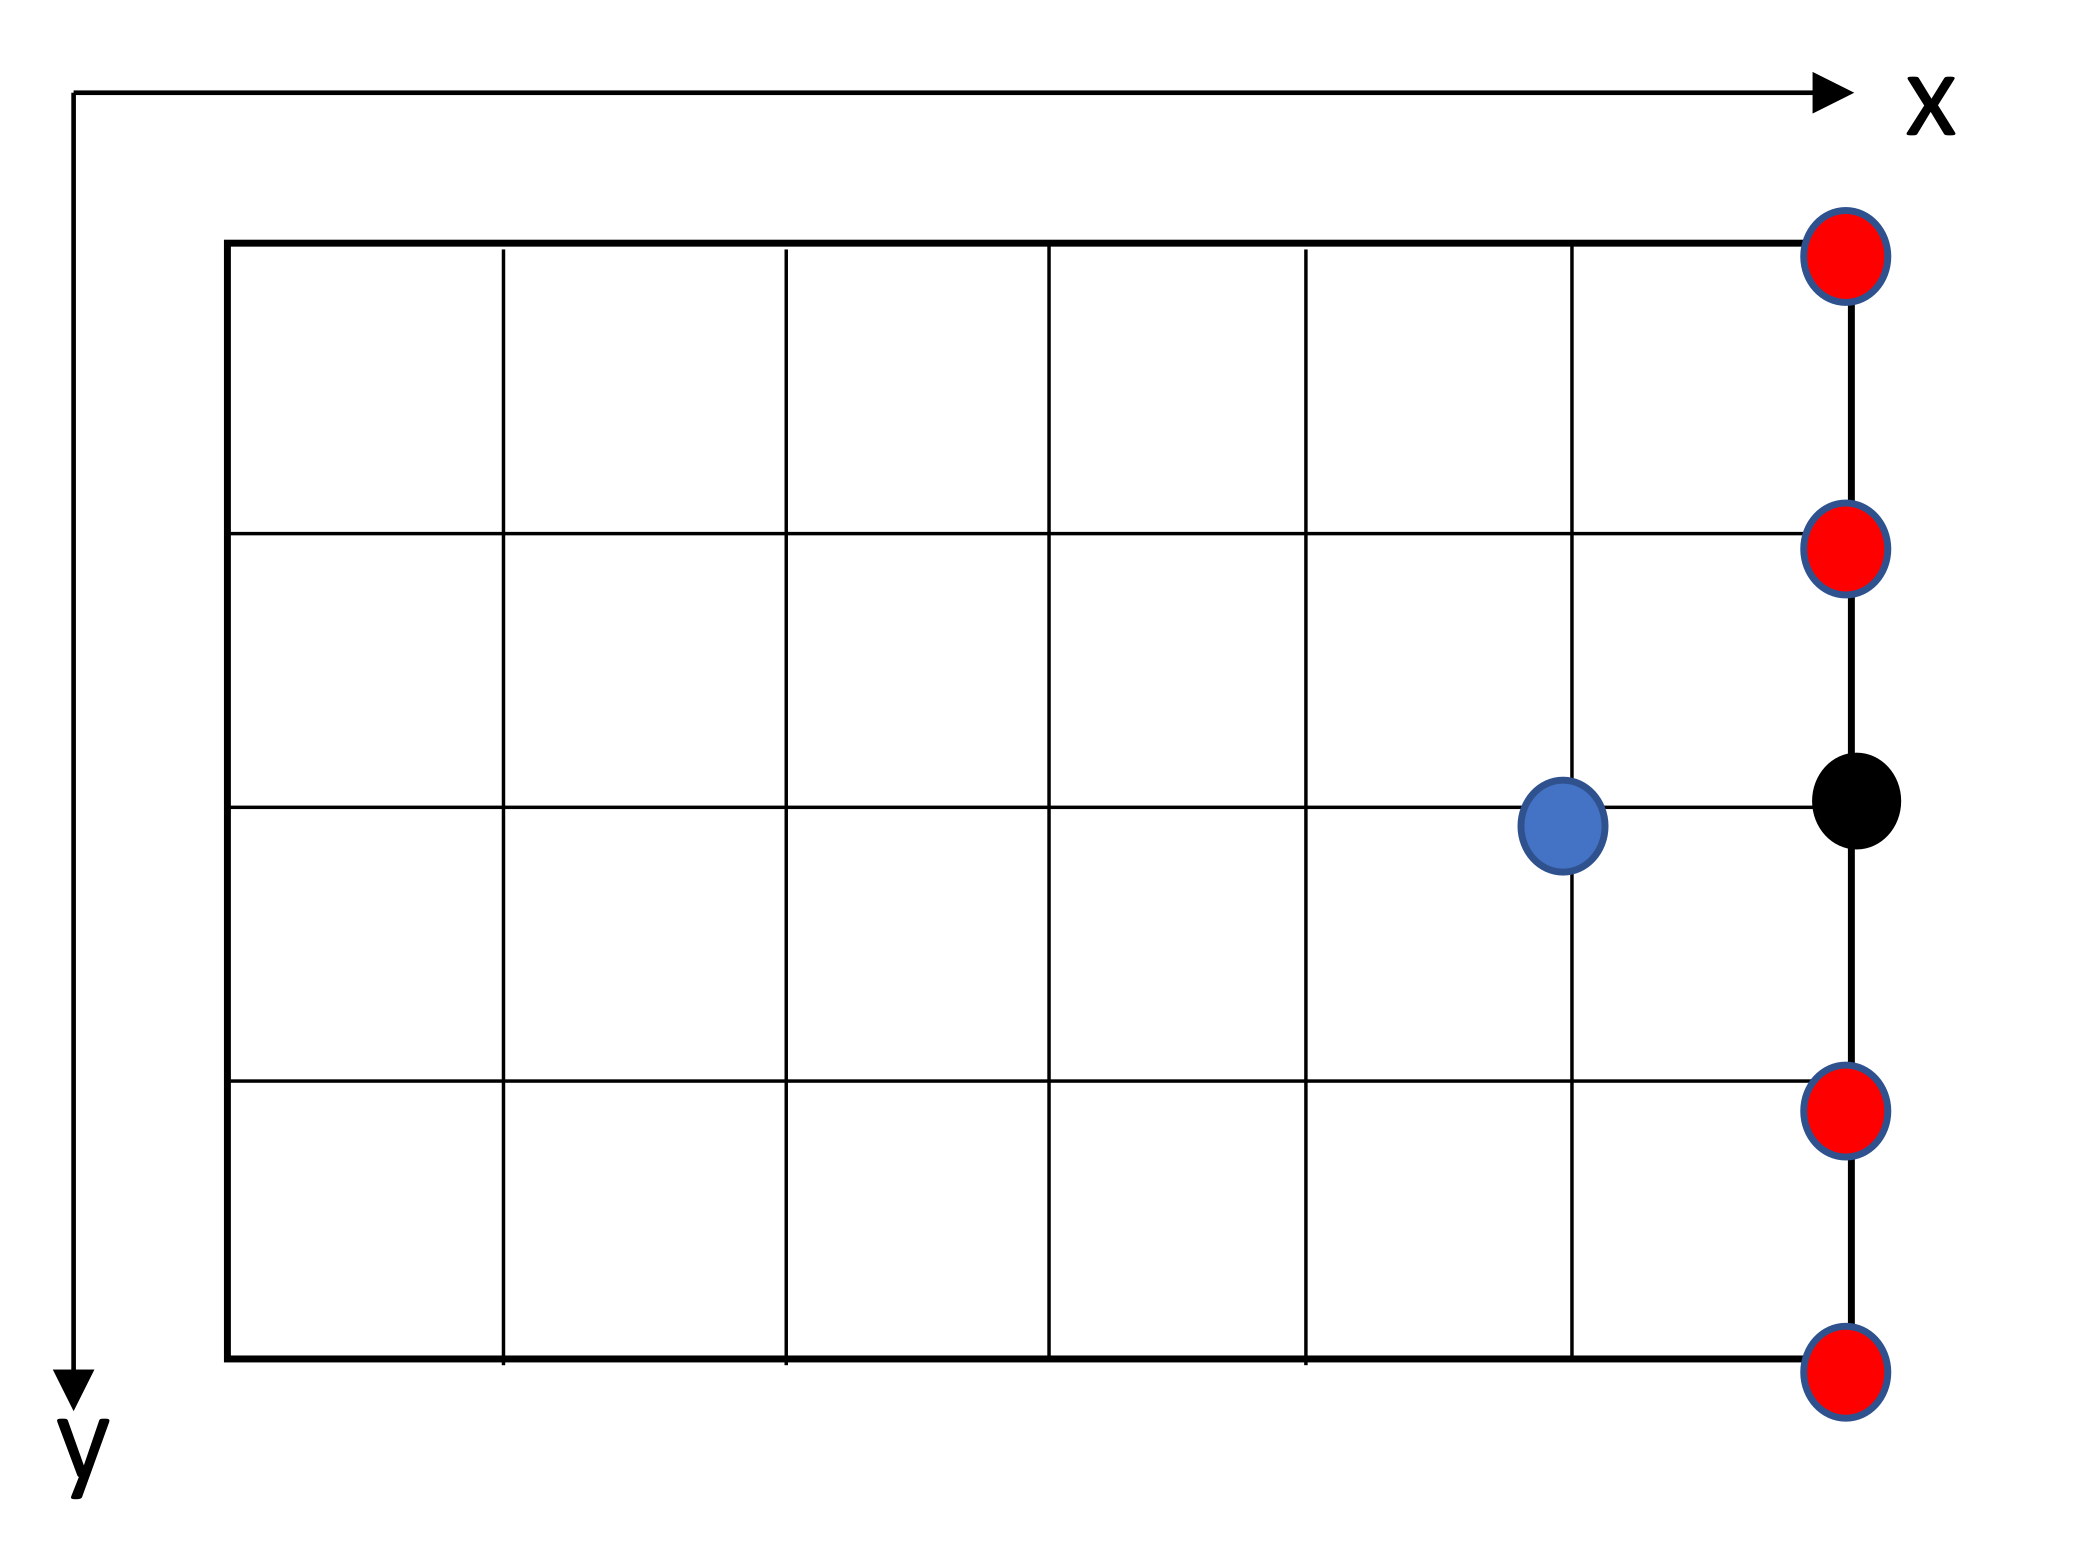
\includegraphics[width=2.5in]{figures/meshborderx2.png}}
    \hspace{1in} 
  \subfigure[$T(2(x_i+2)+1)$]{ 
    \label{fig:subfigmesh2:c} %% label for second subfigure 
    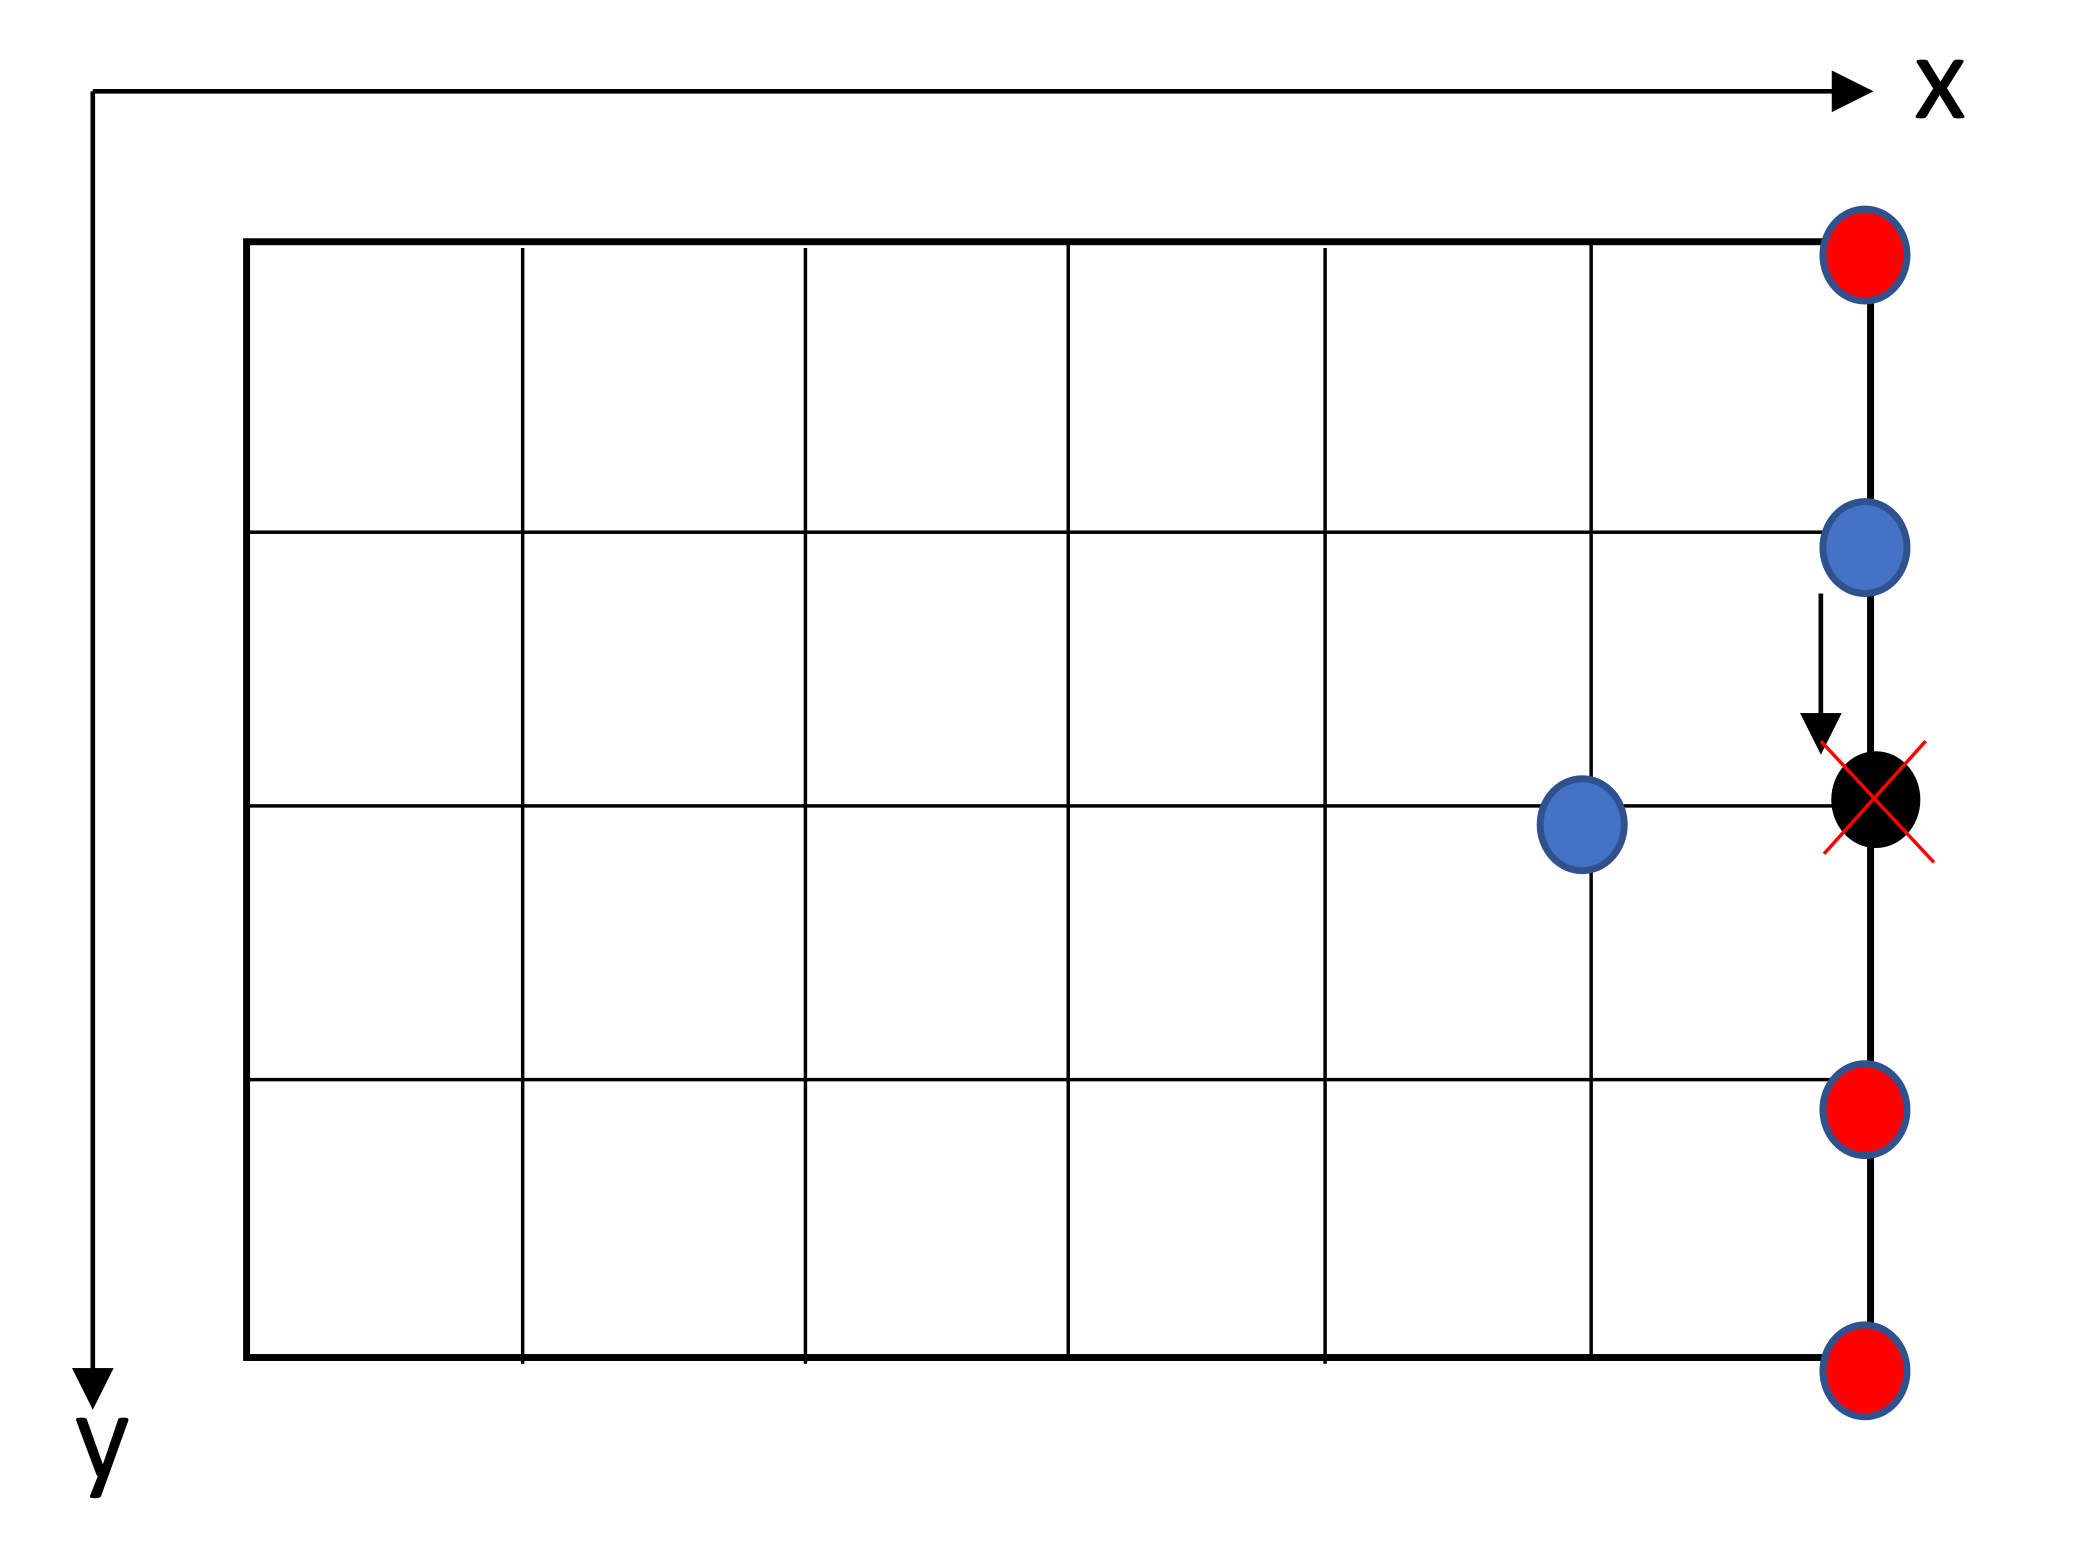
\includegraphics[width=2.5in]{figures/meshborderx3.png}}
%      \hspace{1in} 
    \caption{Arrangement of agents in elimination phase when the new formed BV resides in a border node (when $x=d_1$)} 
  \label{fig:subfigmesh2} %% label for entire figure 
\end{figure}

\item Case 3: When $2<x<d_1$, $y=1$ or $y=d_2-1$ (a border node becomes a new formed BV). For convenience, we only discuss the situation when $y=1$(the solution can be easily modified to fit the scenario when $y=d_2-1$). In this case, agents residing in nodes $(x-1, y+1)$ and $(x-2, y)$ (let's say agents a,b) receive a BV clone at T(2$x_i$+1). Agents $a$ and $b$ move EAST for one step and arrive at node $(x, y+1)$ and node $(x-1, y)$ at T($2(x_i+1)$). Since the number of agents who can be informed of the location of the new formed BV is not enough for decontaminating the BV, we should notify one more agent to participate in the elimination phase. We employ agent $a$ who resides in node $(x, y+1)$ at T(2$x_i$+1) to notify agent residing in node $(x, y+1)$ (let's say agent $c$), so it move NORTH for one step and arrive at node $(x, y+2)$ at T($2(x_i+1)+1$). Then both of agents $a$ and $c$ move SOUTH and reach node $(x, y+1)$ at T($2(x_i+2)$) when the they meet the agent who move from node $(x-1, y+1)$ (let's say agent $d$) and notify it to stop moving. Then agent $a$ move EAST and then SOUTH to reach node $(x+1, y)$ at T($2(x_i+3)$). Finally, at T($2(x_i+3)+1$), agent $d$ move SOUTH to permanently eliminate the BV.

\begin{figure} [H]
  \centering 
  \subfigure[$T(2x_i+1)$]{ 
    \label{fig:subfigmesh3:a} %% label for first subfigure 
    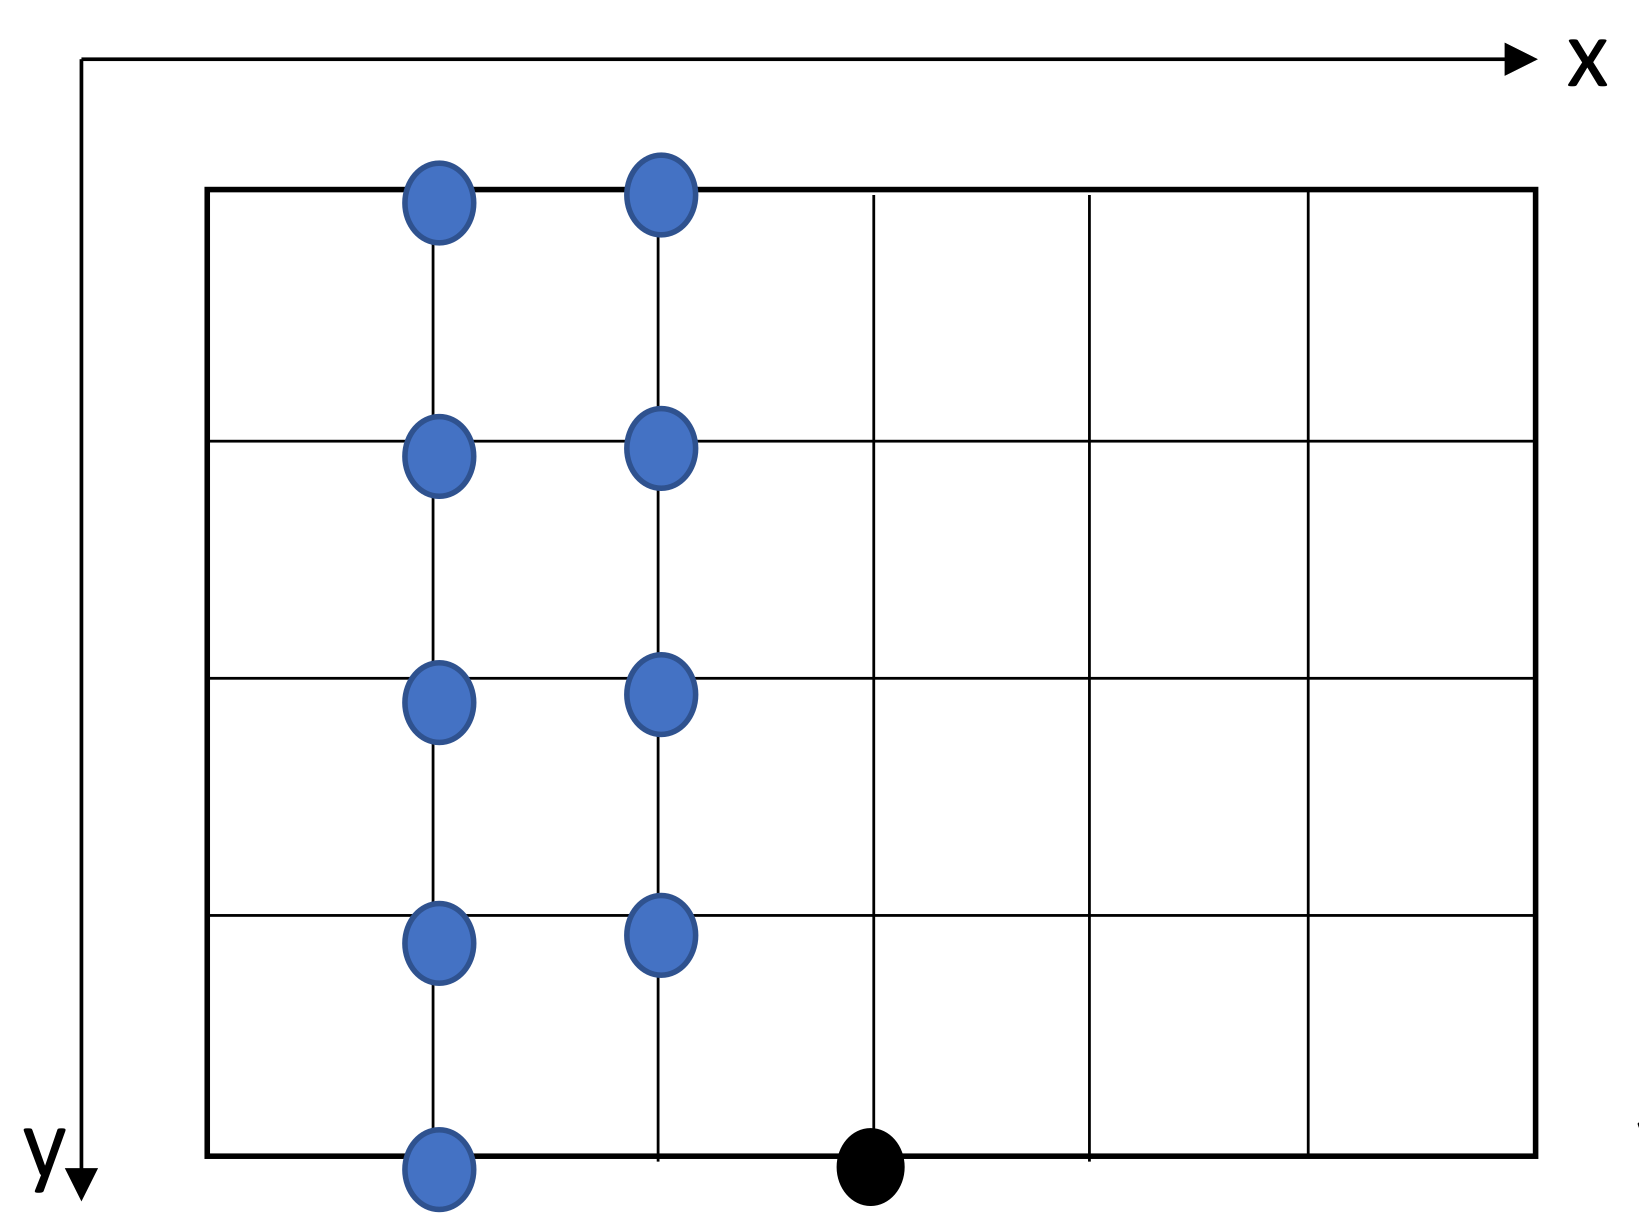
\includegraphics[width=2.5in]{figures/meshbordery1.png}} 
%  \hspace{1in} 
  \subfigure[$T(2(x_i+1))$]{ 
    \label{fig:subfigmesh3:b} %% label for second subfigure 
    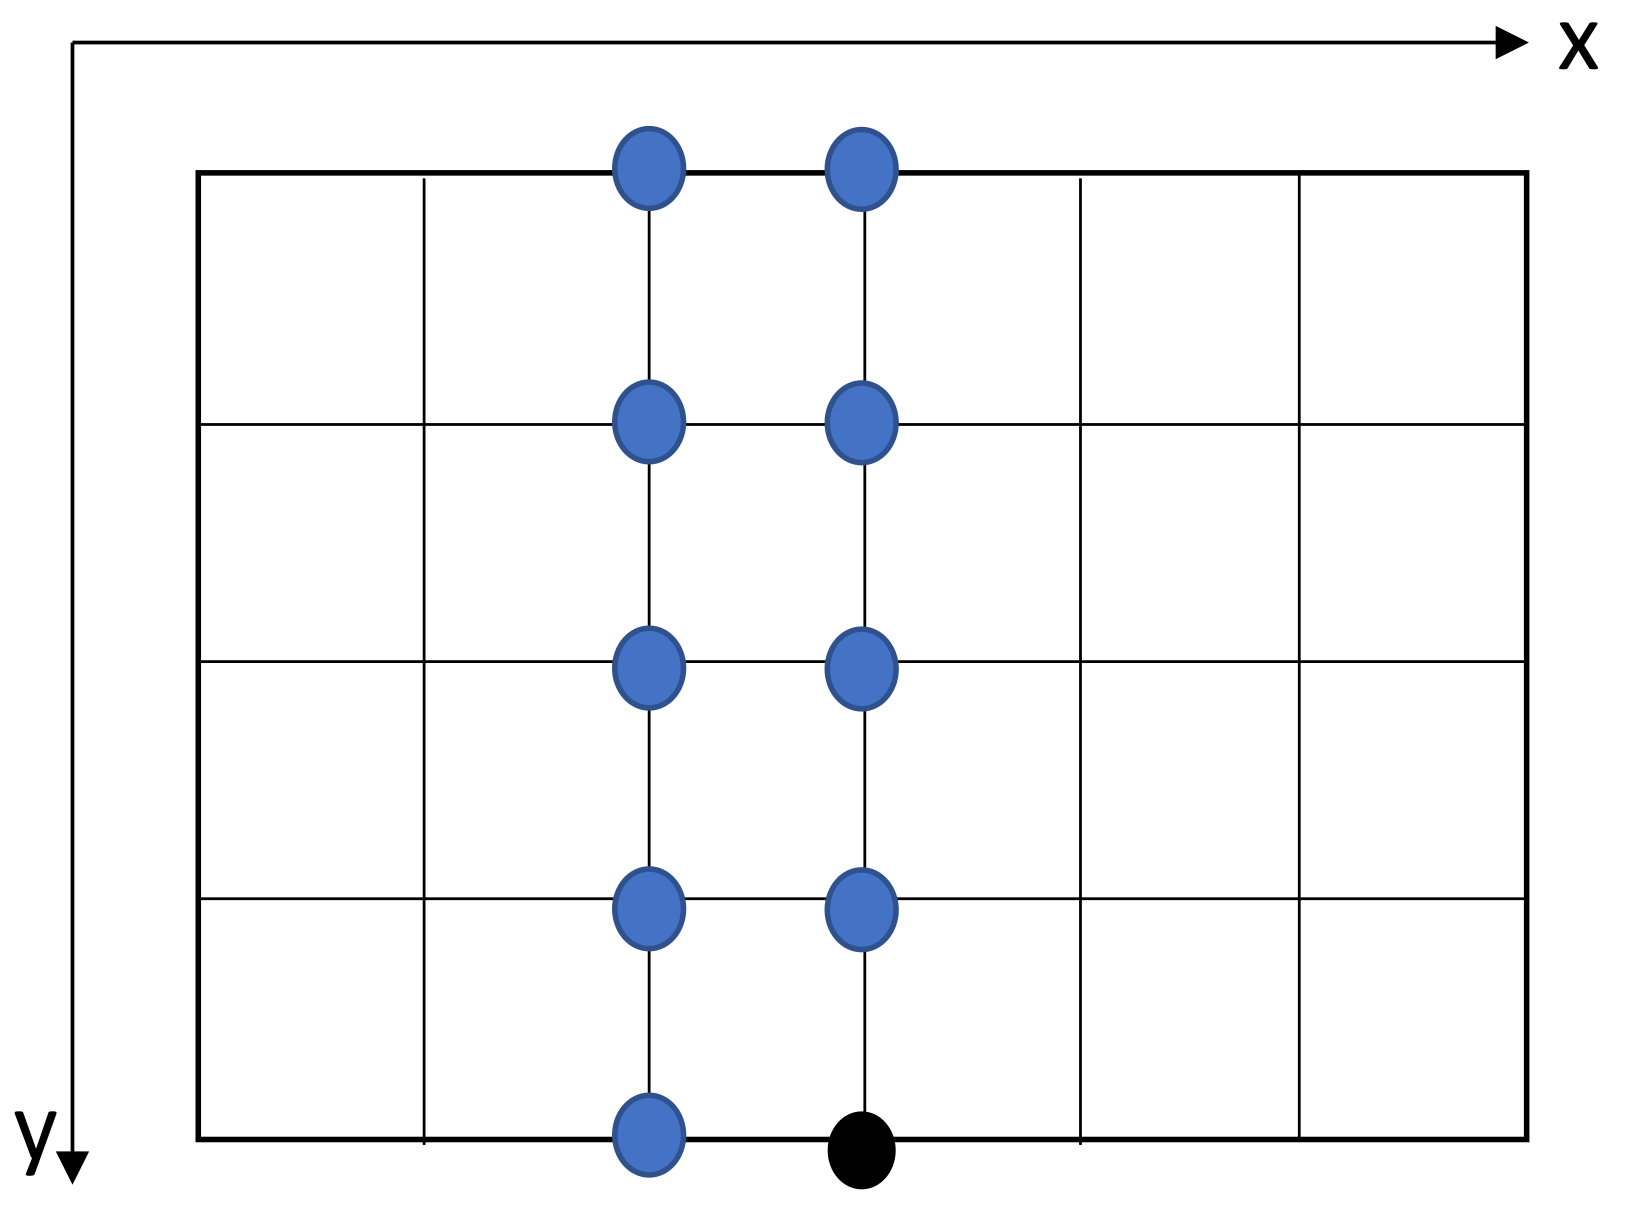
\includegraphics[width=2.5in]{figures/meshbordery2.png}}
    \hspace{1in} 
  \subfigure[$T(2(x_i+2))$]{ 
    \label{fig:subfigmesh3:c} %% label for second subfigure 
    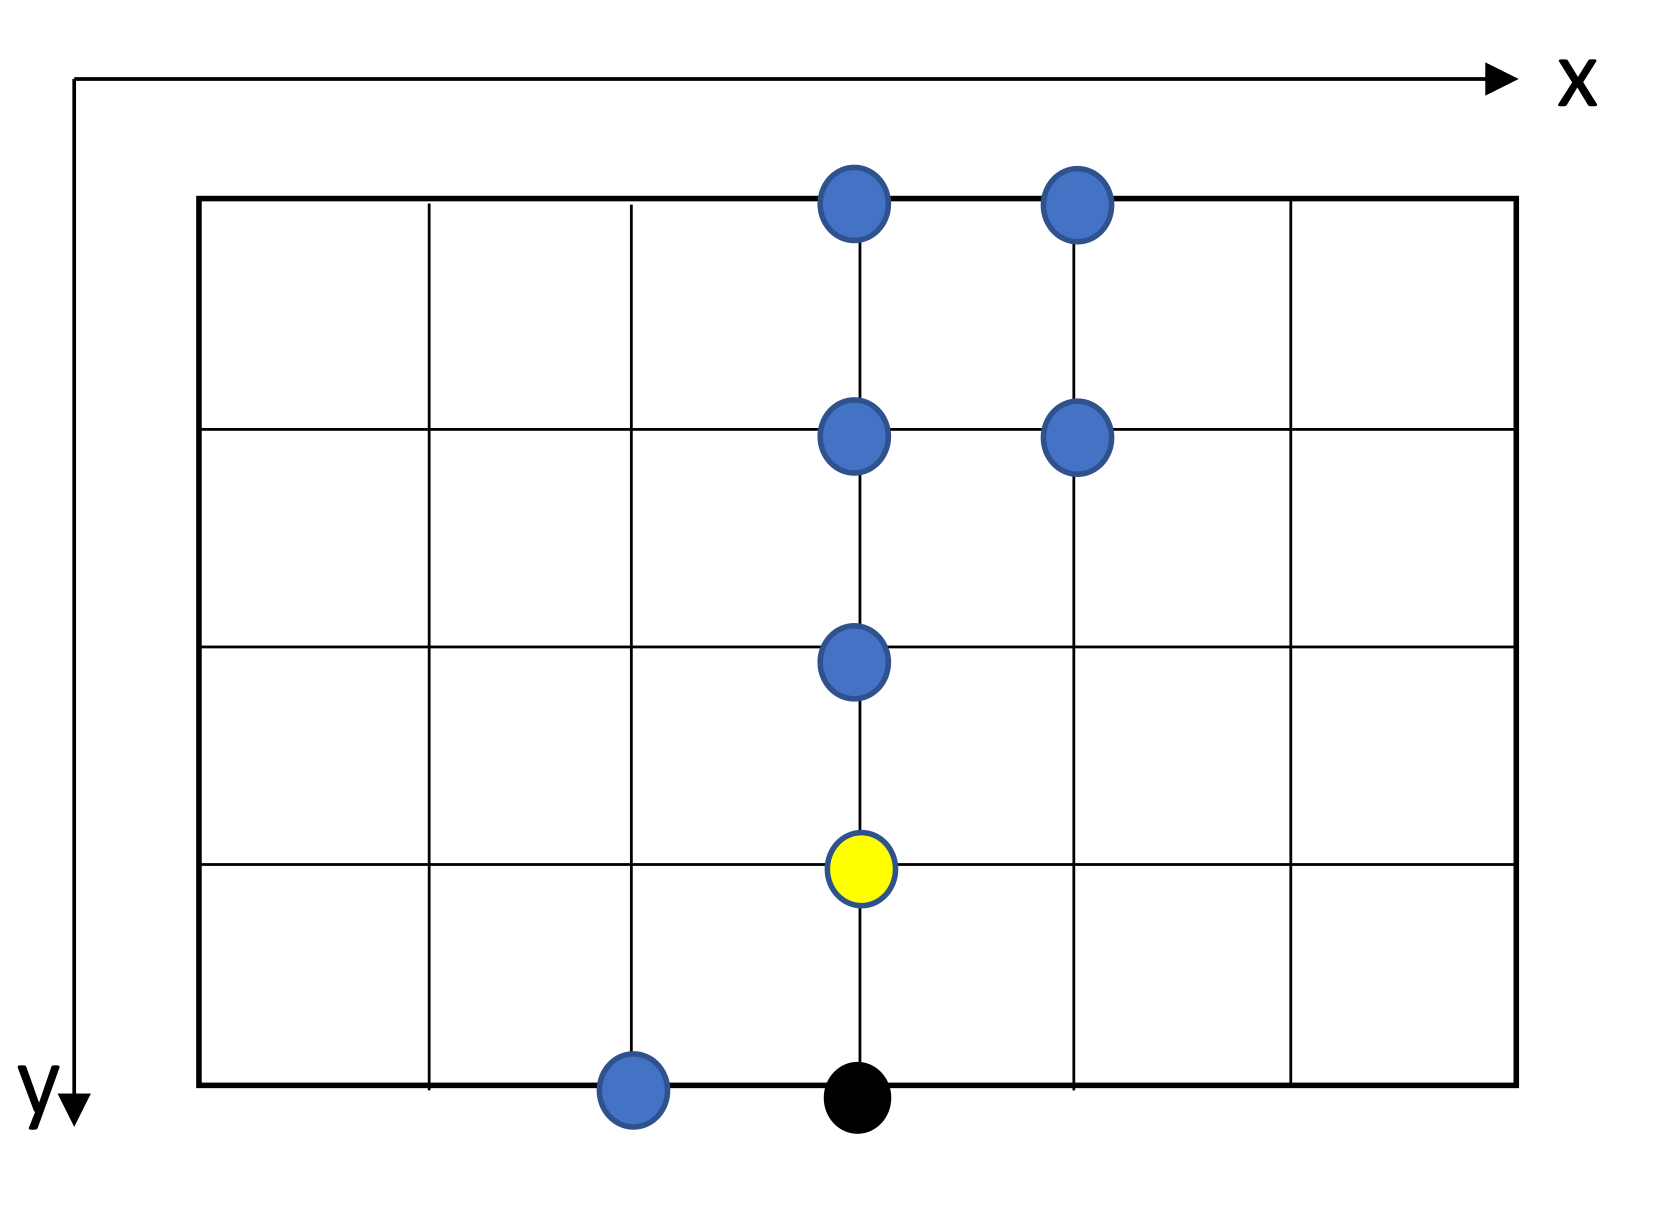
\includegraphics[width=2.5in]{figures/meshbordery3.png}}
%      \hspace{1in} 
  \subfigure[$T(2(x_i+3))$]{ 
    \label{fig:subfigmesh3:d} %% label for second subfigure 
    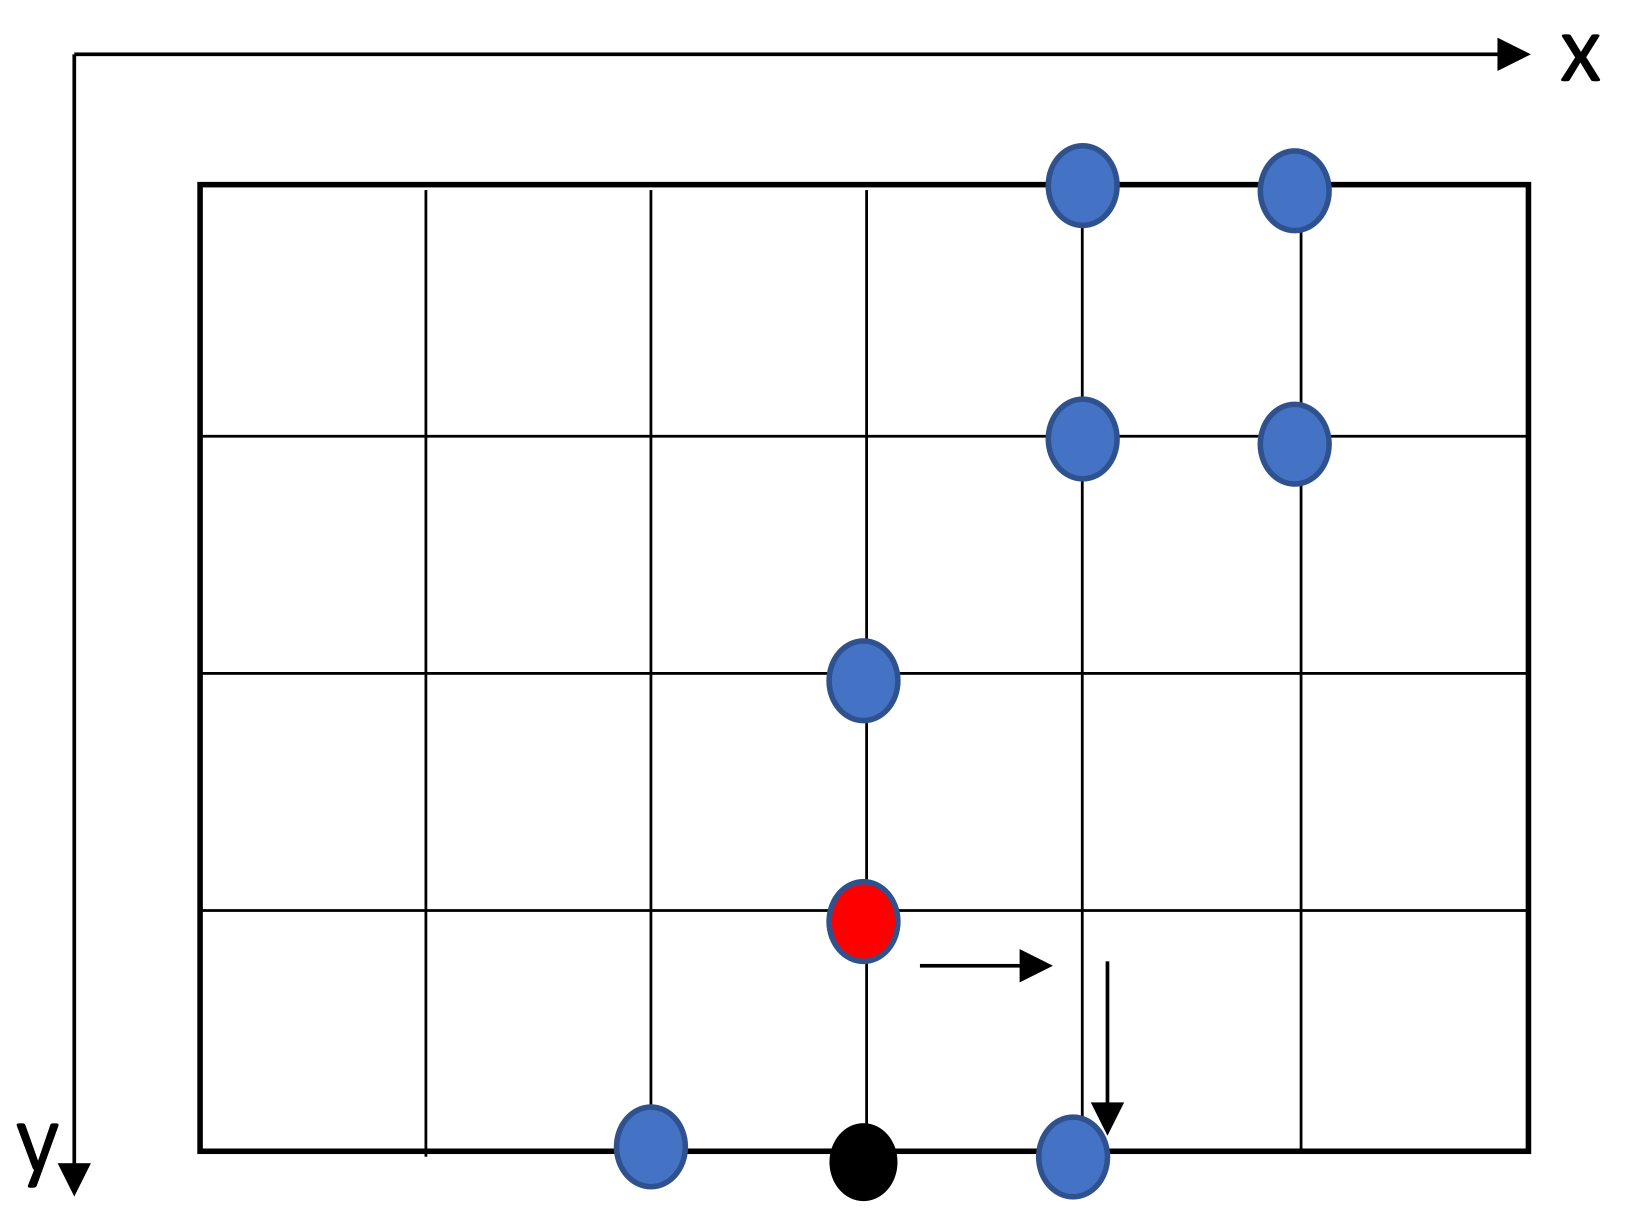
\includegraphics[width=2.5in]{figures/meshbordery4.png}}
      \hspace{1in} 
  \subfigure[$T(2(x_i+3)+1)$]{ 
    \label{fig:subfigmesh3:e} %% label for second subfigure 
    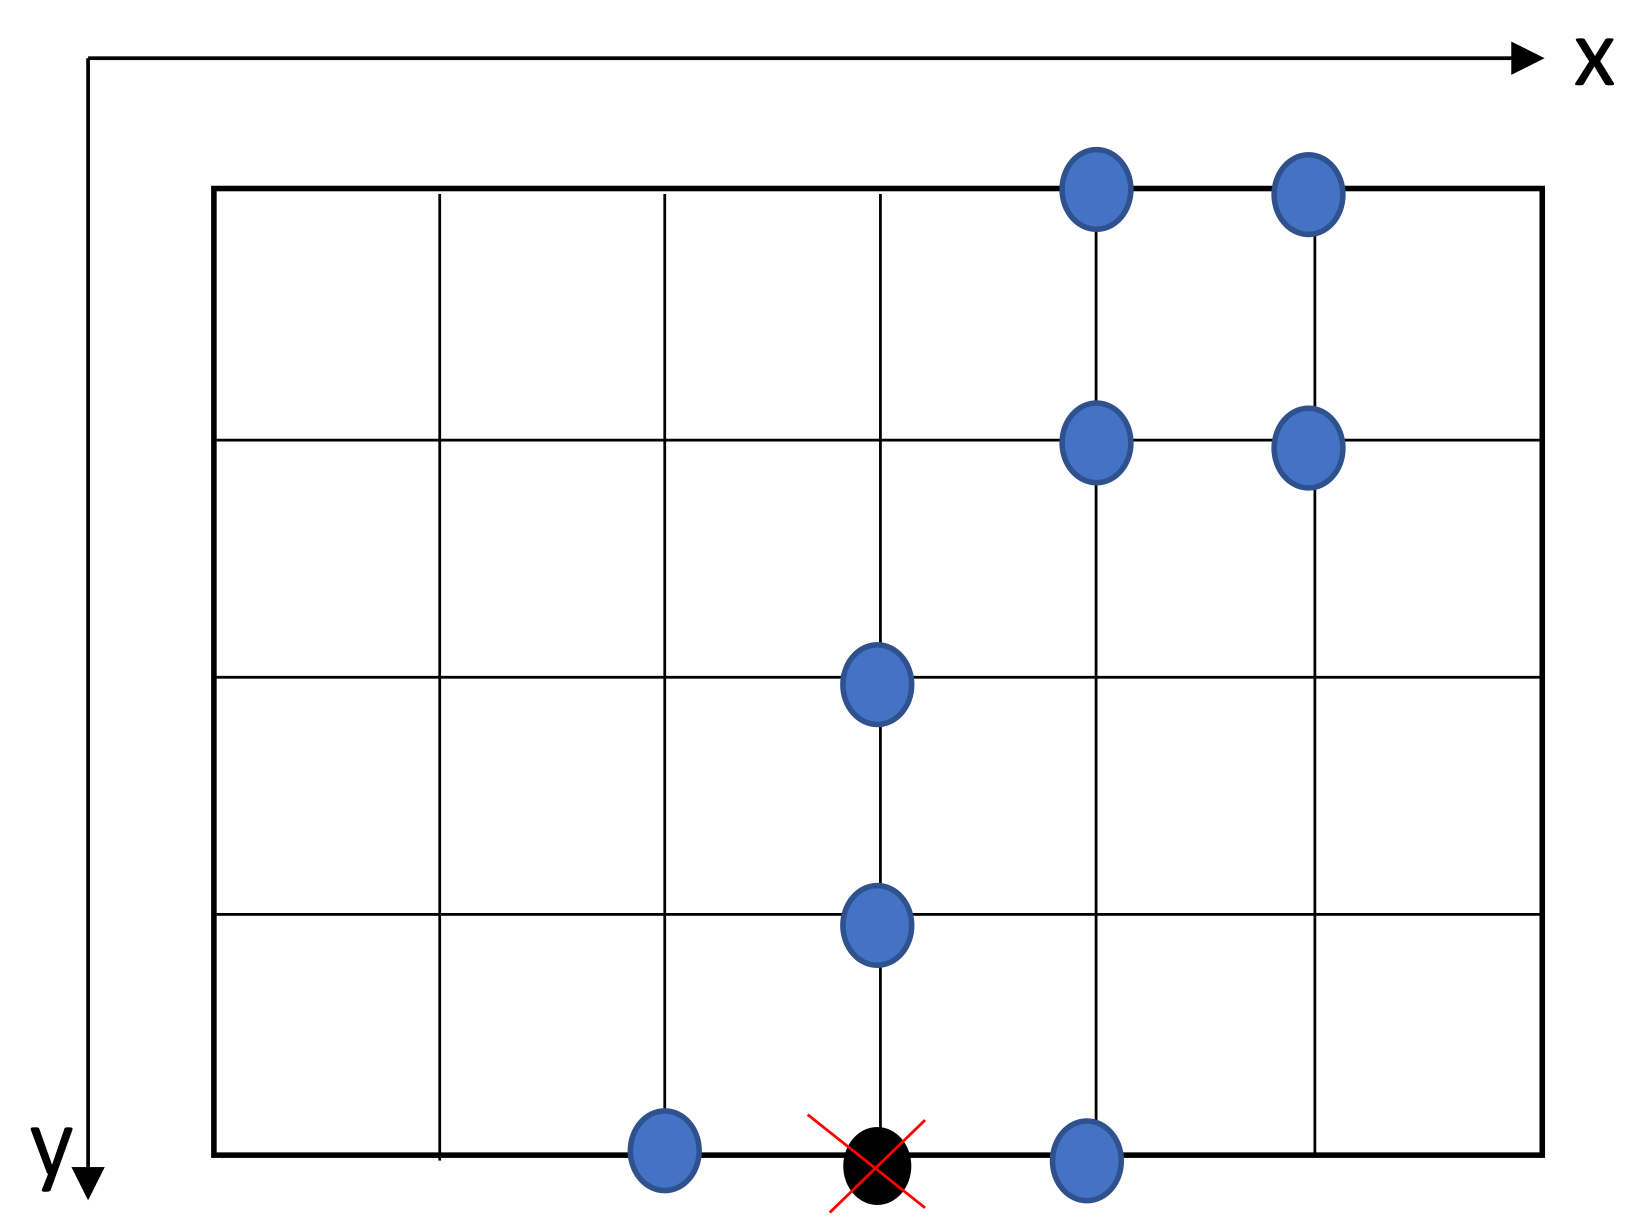
\includegraphics[width=2.5in]{figures/meshbordery5.png}}
  \caption{Arrangement of agents in elimination phase when the new formed BV resides in a border node (when $y=1$ or $y=d_2-1$ ) } 
  \label{fig:subfigmesh3} %% label for entire figure 
\end{figure}

\item Case 4: When $x=d_1$ and $y=1$ or $y=d_2-1$ (a corner node becomes a new formed BV). For convenience, we only discuss the situation when $y=1$. In this case, agents residing in node $(x-1, y+1)$ and $(x-2, y)$ (let's say agents a,b) receive a BV clone at T(2$x_i$+1). Both of them keep moving for one step and arrive at nodes $(x, y+1)$ and $(x-1, y)$ at T$(2(x_i+1))$.
\begin{figure} [H]
  \centering 
  \subfigure[$T(2x_i+1)$]{ 
    \label{fig:subfigmesh4:a} %% label for first subfigure 
    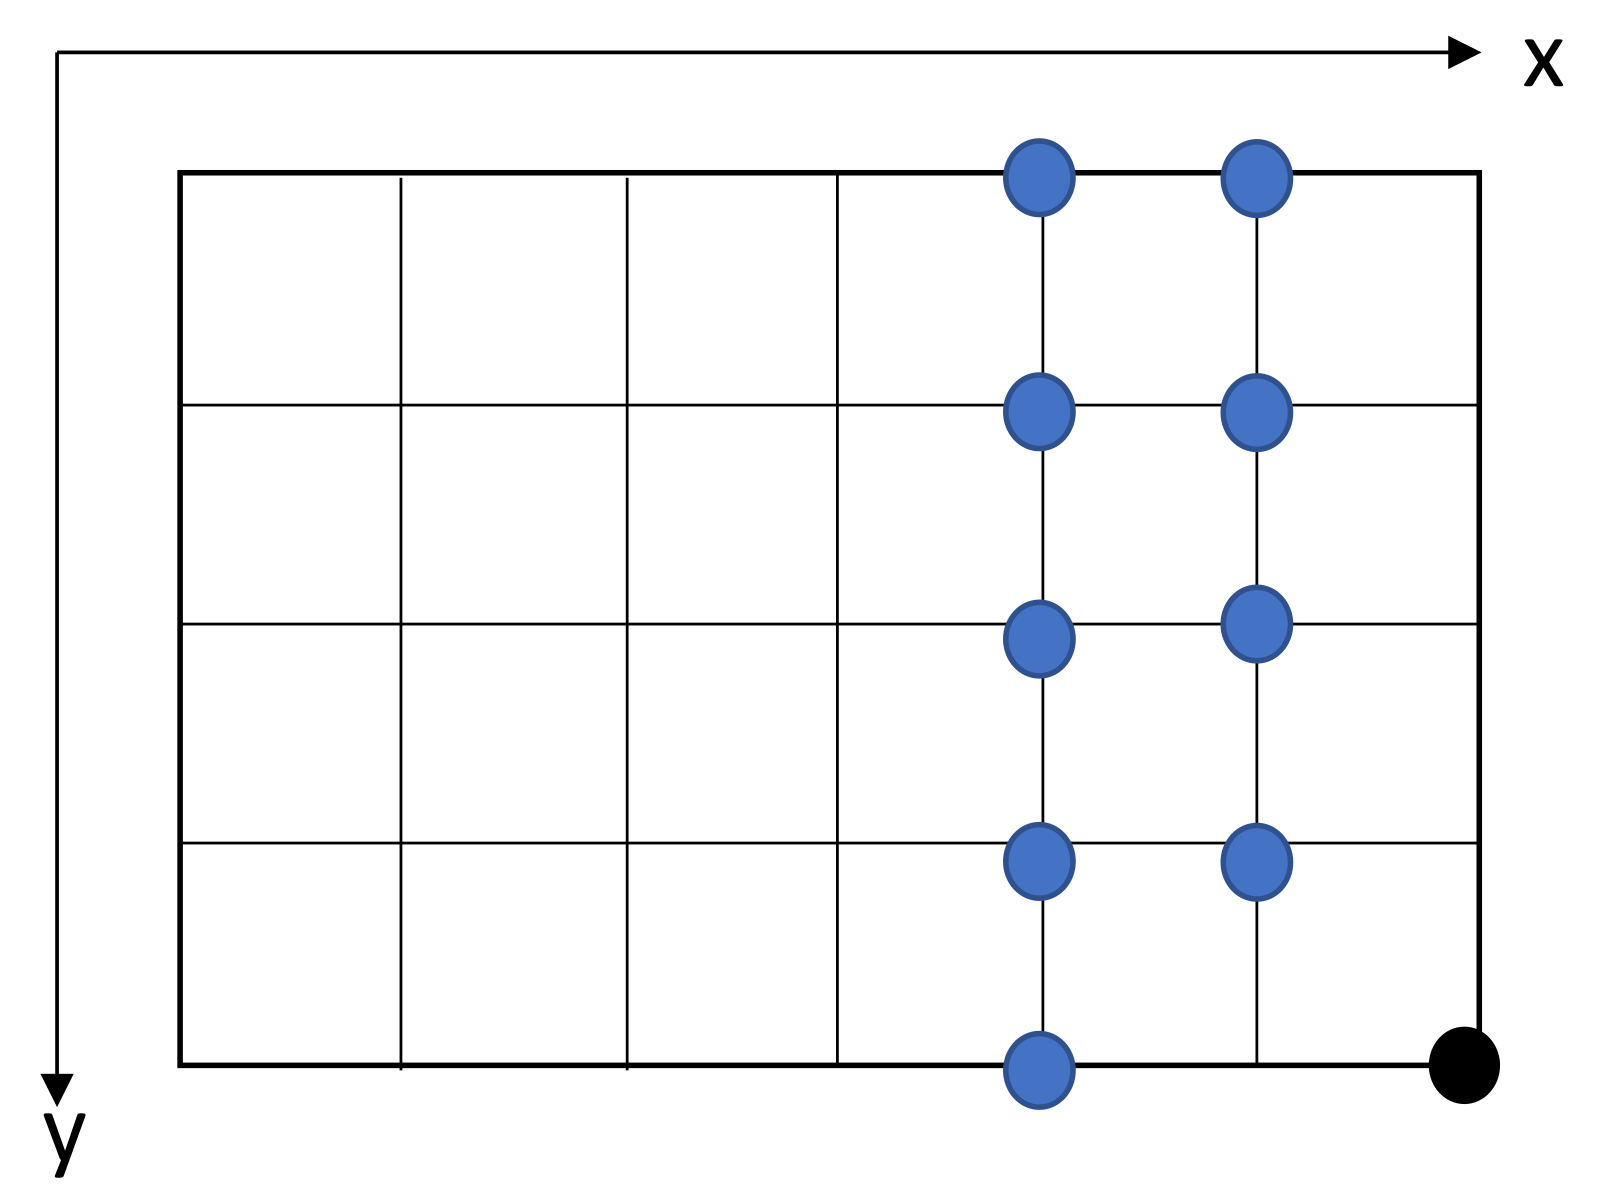
\includegraphics[width=2.5in]{figures/meshcorner1.png}} 
%  \hspace{1in} 
  \subfigure[$T(2(x_i+1))$]{ 
    \label{fig:subfigmesh4:b} %% label for second subfigure 
    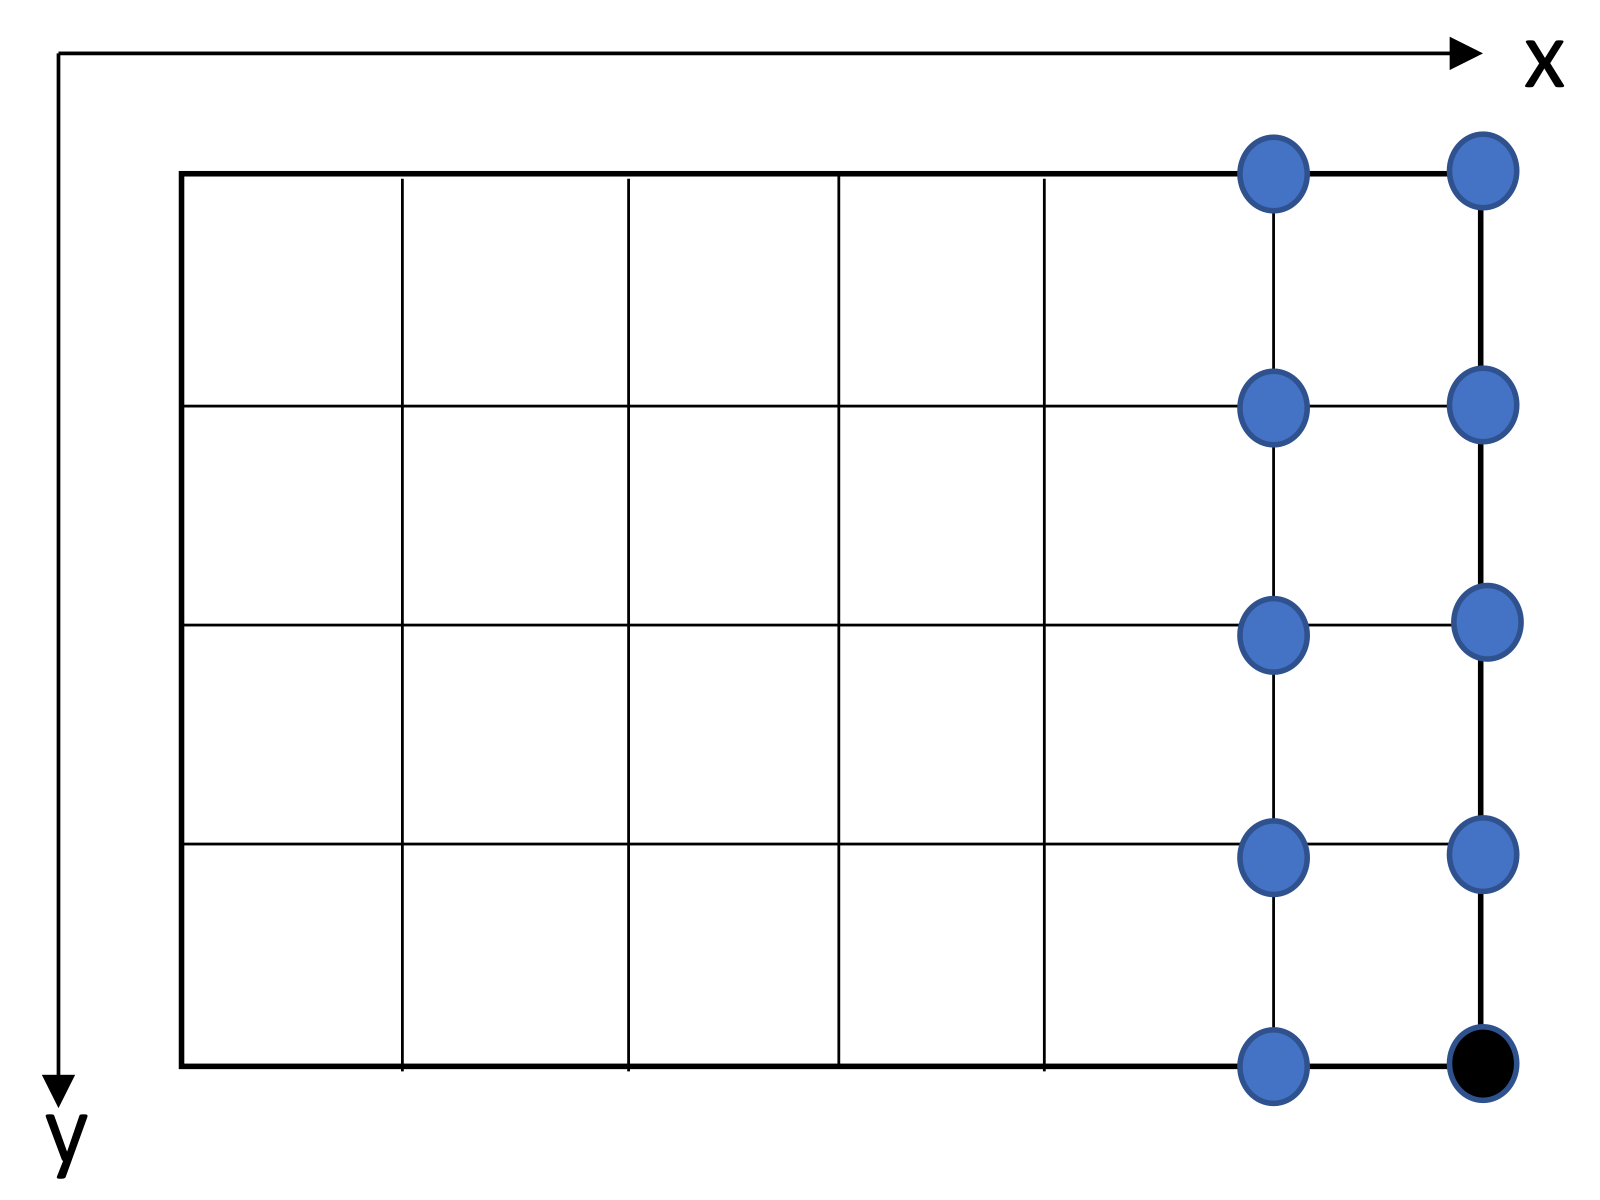
\includegraphics[width=2.5in]{figures/meshcorner2.png}}
    \hspace{1in} 
  \subfigure[$T(2(x_i+2))$]{ 
    \label{fig:subfigmesh4:c} %% label for second subfigure 
    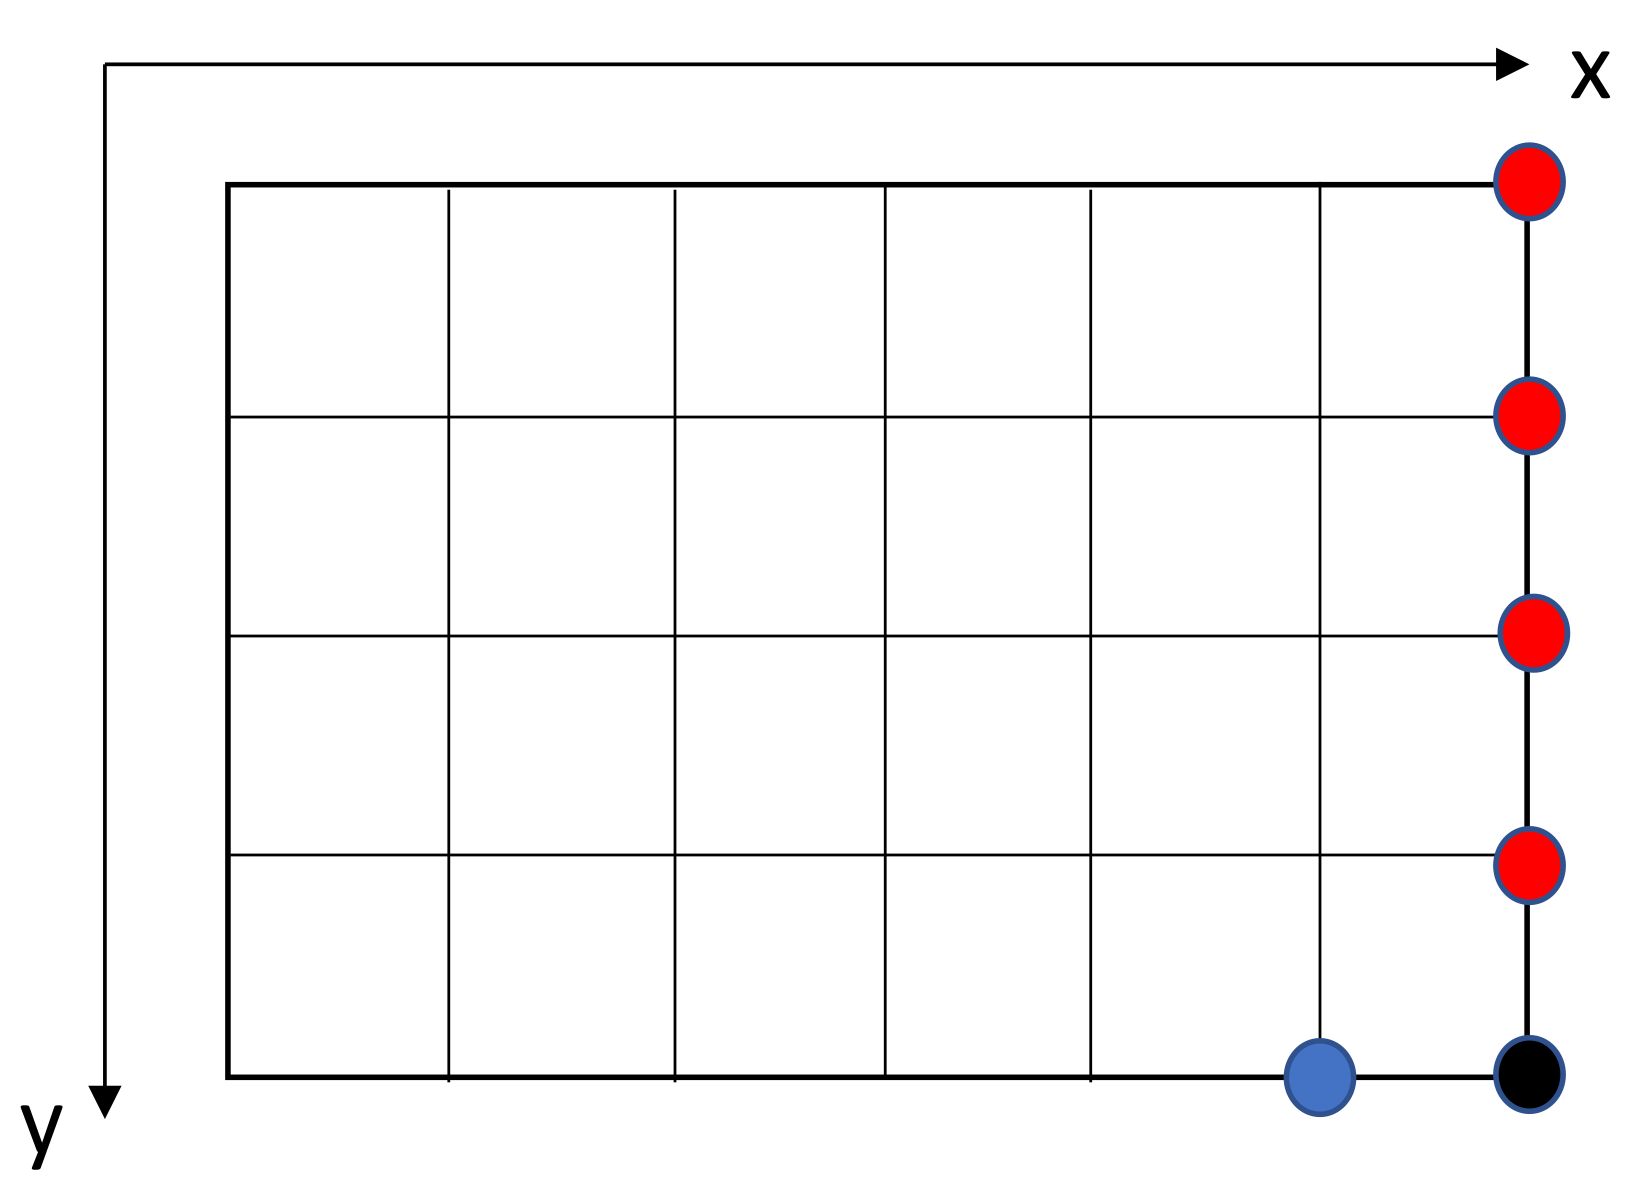
\includegraphics[width=2.5in]{figures/meshcorner3.png}}
%      \hspace{1in} 
\subfigure[$T(2(x_i+2)+1)$]{ 
    \label{fig:subfigmesh4:d} %% label for second subfigure 
    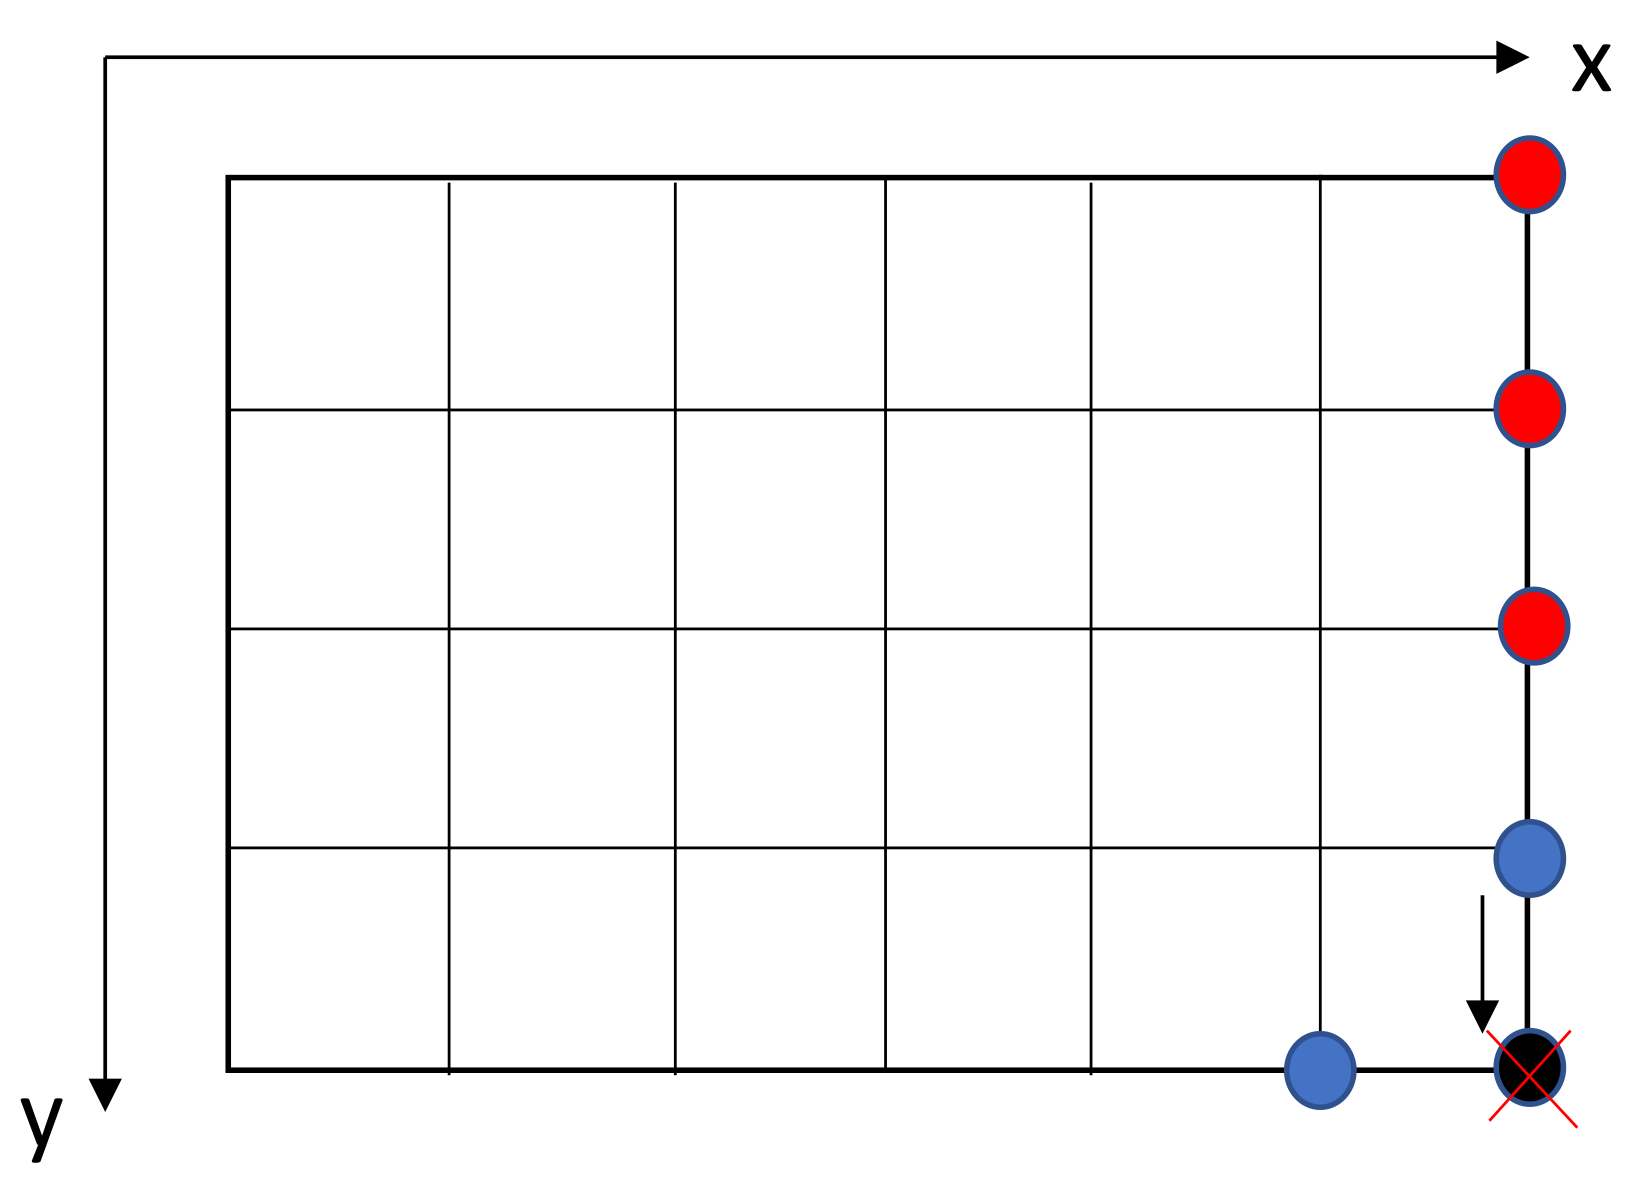
\includegraphics[width=2.5in]{figures/meshcorner4.png}}
    \caption{Arrangement of agents in elimination phase when the new formed BV resides in a corner (when $x=d_1$ and $y=1$ or $y=d_2-1$)} 
  \label{fig:subfigmesh4} %% label for entire figure 
\end{figure}
\end{itemize}

\noindent{\bf Analysis and Comparing}
\begin{theorem}
Mesh contamination algorithm performs a decontamination of a mesh (size of $n=d_1\times d_2(d_1>2,d_2>2)$ using $k=2\sqrt{n}$ agents and at most 1 casualties.
\end{theorem}
\begin{proof}
Let $v=(x, y)$ be the node containing the BV. When one of the agent in the exploring group moves to $v$, it will be destroyed and the BV will move to all neighbours of $v$. If $x=1$, then the neighbours $(x, y+1)$, $(x, y-1)$ and $(x+1, y)$ are protected by agents and neighbour $(x-1, y)$ actually does not exist; if $x>1$, then neighbours $(x, y+1)$, $(x, y-1)$ and $(x-1, y)$ are protected by agents. So when the clones of BV moves to the neighbours of $v$, those contain a agent will not be infected by the BV clone; this means that the BV can safely move only to the unexplored neighbours of $v$, of which are at most one. In other words, after $v$ is explored, at most one BV node are formed. According to our elimination strategy, the new formed BV node can be surrounded and destroyed using at most five agents: one to enter a BV and four to protect the neighbours. Since we have one new formed BV, the number of agents participating in the elimination phase is at most five. In addition to the agent destroyed by the original BV, the number of agent needed to complete the elimination phase is at least six. Since we employ $k=2d_1$ ($d_1\geq 3$) which means at the beginning we have at least six agents, so $2d_1$ agents are enough for the decontamination algorithm.
\end{proof}
Let us now consider the number of movements.
\begin{theorem}
Parallel mesh decontamination algorithm performs a BV decontamination of a mesh of size n with at most $2n-\sqrt{n}+O(1)$ movements in time at most $\sqrt{n}+11$.
\end{theorem}
\begin{proof}
Let $v=(x, y)$ be the BV node, and let the size of the grid be $n=d_1\times d_2$. Let us first consider the number of movements performed during the shadowed exploration. Since all the agents simply move EAST at the beginning of T(2n) ($n=0,1, \dots , d_2-1$), the travelling distance is $x$ for agents in the exploring group ({em EA}) and $x-1$ for agents in the shadowing group({em SA}). We have $d_1$ {\em EAs} and $d_1$ {\em SAs}, then we have an overall cost of at most $d_1\times (2x-1)$ movements for this phase.
Consider now the number of movements performed for Surrounding and Elimination. In this part, we only compute the movements of the agents who participate in the Surrounding and Elimination. More specifically, we simply ignore the movements of the agents who do not know the existence of the BV in the whole process. As we discuss in the Elimination phase, when the new formed BV is located in a interior node, ten movements are needed in this phase; when the new formed BV is located in a border node (let' s say $(a, b)$), then eight movements are needed when $a=d_1, 2< b <d_2-1$ and eleven movements are needed when $2< a <d_1,b=1 or b=d_2-1$; when the new formed BV is located in a corner node, then five movements are needed in this phase. Hence $O(1)$ movements are performed in this phase.
In total we have that the number of movements is at most $d_1 \times(2x-1)+O(1)\leq \sqrt{n}\times(2\sqrt{n}-1)+O(1)$, which is $2n-\sqrt{n}+O(1)$.\\
As for the time complexity. The time required for the exploration phase is equal to the number of movements of EA, which is $d_1$; the time required for the surrounding and elimination phase is at most eleven. So in total the parallel mesh decontamination algorithm terminate in time at most $\sqrt{n}+11$. 
\end{proof}

Now we make some comparison between our strategy and the sequential strategy.

\begin{table} [hbtp]
\caption{Appointment Card}
\label{table:AptCard}
\centering
\tabulinesep=2mm
\begin{tabu} to 140 mm {|X[6,c]|X[4,l]|X[4,l]|X[4,l]|X[4,l]|} \hline 
%\begin{tabular}{|c|l|} \hline 
& The number of agent & The time cost & The number of movement & The casualties \\ \hline
{\em PBVD-2G}   & $2\sqrt{n}$   & $\sqrt{n}+11$ & $2n-\sqrt{n}+O(1)$   & 1        \\ \hline
{\em BVD-2G} & 7    & $3n$          & $9n+O(1)$     & 3              \\ \hline
\end{tabu}
%\end{tabular}
\end{table}

\subsection{Multi-Dimensional Grid}
Let $M$ be a q-dimensional grid of size $d_1\times\ldots\times d_q$ and let each node of $M$ be denoted by its coordinates $(x_1,\ldots,x_q)$, $1\leq x_i\leq d_i$. The algorithm, called {\em PBVD-qG}, follows a general strategy similar to the one described in Section 4.2.1: a safe exploration with shadowing, followed by a surrounding and elimination phase. 









